%Koma-Script book mit Bindekorrektur
%DIV - wirkt sich auf die Satzspiegelma�e aus
%cleardoubleempty - zeigt keine Kopf- und Fu�zeile bei leeren Seiten an (nur Seitenanzahl: cleardoubleplain)
%headsepline - Linie unter der Kopfzeile
%chapterprefix - schreibt Chapter II und dann Titel, anstatt nur Titel
%liststotoc - Inhaltsverzeichnis nimmt auch Tabellen- und Bildverzeichnis auf
%bibtotoc - �hnlich, nur mit Literaturverzeichnis
%openbib - cooleres Literaturverzeichnislayout
%draft oder final - zeigt die Graphiken nicht an und markiert overfull boxes
\documentclass[paper=a4,fontsize=11pt,twoside,BCOR8.25mm, DIV9,
cleardoublepage=empty, headsepline, chapterprefix]{scrbook}

%Regelt den Zeilenabstand
\usepackage{setspace}
\onehalfspacing

%Hurenkinder und Schusterjungen vermeiden
\clubpenalty = 10000
\widowpenalty = 10000 \displaywidowpenalty = 10000
\setlength{\headheight}{1.15\baselineskip}

\usepackage[latin1]{inputenc} %f�r die Umlaute und das �
\usepackage{scrpage2} %Kopf und Fu�zeilen - k�nnen definiert werden
\usepackage{graphicx}
\usepackage{enumitem}
\usepackage{array} %Tabellen
\pagestyle{scrheadings}
\setheadtopline{1pt}

\usepackage{fancybox} %F�r Boxenumrahmungen
 
%commands
\newcommand{\bfitem}[1]{\item \textbf{#1}}
\newcommand{\para}[1]{\vskip 15pt \textbf{#1}\hskip 15pt}

\newcommand{\msQuote}[2]{
\begin{quote}
    \noindent\itshape\small
    ``#1" \\\- \hspace{\fill}#2
\end{quote}}
  
\setlength{\parskip}{5pt} %Abstand zwischen Paragraphen


\usepackage{amssymb} %F�r Mathe-Symbole
\usepackage{amsmath}
\usepackage{rotating}

%-------------------------------------------

\begin{document}

\begin{titlepage}
\sffamily
\hskip 1cm

\includegraphics[width=3cm]{Bilder/unilogo}
	\vskip -6.15cm 
	\hskip 4.3cm
	\rule{1pt}{5.93cm}
	\hskip 0.1cm
	\vbox{ \hsize=8cm \raggedright
		\textsc{\LARGE
			Leopold-Franzens\\
			University of Innsbruck\\
			\bigskip \Large
			Institute of\\ 
			Computer Science\\
			\bigskip \large 
			Research Group\\ 
			Quality Engineering
		 }
	 }

\begin{center} 
%
\vskip 0.8cm
%
\textsc{\Large Master Thesis}
%
\vskip 2.2cm
%
\vbox{
%
{\bfseries\textsf{\huge
	Enhanced Mashup and Application Composition based on OSGi
}}
%
}
%
\vfill
%
% split the page into two columns
% left column
\begin{minipage}{0.4\textwidth}
\begin{flushleft}
Author\\
\textbf{Felix Sch�pf Bakk.techn.}\\
\end{flushleft}
\end{minipage}
%
% right column
\begin{minipage}{0.4\textwidth}
\begin{flushright}
Supervisor\\
\textbf{Dr. Barbara Weber}\\
\end{flushright}
\end{minipage}
%
\vskip 1cm
%
\today
%
\end{center}
\thispagestyle{empty}
\end{titlepage}

\cleardoublepage
\thispagestyle{empty}
\vskip 1cm
\begin{center}{\huge\bfseries Acknowledgment}\end{center}
\vskip 2cm
\normalsize

\addcontentsline{toc}{chapter}{Acknowledgment}

\noindent I would like to thank my supervisor, \textbf{Priv.-Doz. Dr. Barbara Weber}, for her
encouragement, support and feedback from the initial to the final level. Her valuable guidance and advices enabled
the development of the powerful Component Framework and therewith the completion of this thesis.

\bigskip \noindent Furthermore, I want to thank all people who detected shortcomings within the
thesis as well as the implemented framework. Special thank goes to \textbf{Mathias Breu�} who based
his bachelor thesis on the Component Framework and therefore provided valuable feedback and ideas
for improvement.

\bigskip \noindent Last but not least I want to thank \textbf{my familiy} and \textbf{my girlfriend}
for their appreciation and their continuous support during the entire study. They cheered me up in
hard times and celebrated the achieved milestones, which made them more valuable for me.

\cleardoublepage
\thispagestyle{empty}
\begin{center}
\huge \textbf{Abstract}
\end{center}
\vskip 2cm

\noindent Software products which are used within business are often utilized within different
business processes and by different users within different roles and hence should be flexible and
adaptable to different requirements. Therefore, this thesis evaluates so-called ``Mashup Composers''
which provide an interface to combine the nearly infinite number of data sources exhibited by the
world wide web. These tools introduce the necessary flexible service oriented approach and therewith
enable the combination and aggregation of multiple different services into a single application
without the need for any programming skills.

Yet, the evaluated software products are mainly applicable for monitoring purposes and lack some
essential functionalities, like hot deployment, grouping of blocks, event management and a logging
mechanism, to create powerful applications -- hence, the ``Component Framework'' was implemented.
Based on approved technologies like Java and OSGi this prototype framework provides an infrastructure
for developing, managing, displaying and connecting so-called components. To demonstrate the
feasibility of the framework a test application was implemented which provides an interface to this
framework and enables the composition of simple mashups and applications respectively by dragging and
dropping the various components onto a working area and connecting them.

\cleardoublepage
\thispagestyle{empty}
\vskip 1cm
\begin{center}{\huge\bfseries Declaration of Authorship}\end{center}
\vskip 2cm
\normalsize

\addcontentsline{toc}{chapter}{Declaration of Authorship}

\noindent 
I, Felix Sch�pf Bakk.techn., declare that this thesis and the work
presented in it are my own. I confirm that:

\begin{itemize} 
	\item[\tiny{$\blacksquare$}] This work was done wholly while in
candidature for a research degree at this University.
 
	\item[\tiny{$\blacksquare$}] No part of this thesis has previously
	been submitted for a degree or any other qualification at this University or any other
institution.
 
	\item[\tiny{$\blacksquare$}] Where I have consulted the published work of
others, this is always clearly attributed.

	\item[\tiny{$\blacksquare$}] Where I have quoted from the work of others, the
source is always given. With the exception of such quotations, this thesis is
entirely my own work.
 
	\item[\tiny{$\blacksquare$}] I have acknowledged all main sources of help.
 
	\item[\tiny{$\blacksquare$}] Where the thesis is based on work done by myself
jointly with others, I have made clear exactly what was done by others and what I
have contributed myself.
\end{itemize}
%
\vskip 3.5cm
%
\begin{minipage}{0.42\textwidth}
	\raggedright
	\rule{0.8\textwidth}{0.5pt}\\
	\vskip -2mm
	\small Date
\end{minipage}
%
\hfill
%
\begin{minipage}{0.5\textwidth}
	\raggedright
	\rule{\textwidth}{0.5pt}\\
	\vskip -2mm
	\small Signature
	\hfill
	(Felix Sch�pf)
\end{minipage}
%
%
\cleardoublepage

\setcounter{page}{1}
\pagenumbering{roman}
\tableofcontents
\cleardoublepage

\setcounter{page}{1}
\pagenumbering{arabic}

\chapter{Introduction}
\label{chapter:introduction}

Nowadays companies have to be increasingly flexible due to a fast changing market in order to remain
competitive. Hence, business processes have to be highly adaptable and extensible to the current
market requirements. Furthermore, most business processes within modern companies rely on various
different software products which therefore have to be easily adaptable as well. This statement is
emphasised by \cite{flexible_software}:

\msQuote{Most executives say that their businesses are changing faster than their IT organizations
can keep critical systems current. Yet IT cannot afford to make any major modifications because so
much of the technology budget is devoted to incremental maintenance.}

To base a software product on a service oriented architecture constitutes one possibility to support
the flexibility and adaptability requirements. Furthermore, this architecture can be provided with an
interface, which enables the dynamic combination and orchestration of services without any
programming skills, similar to ``Mashup Composers''. These mashup composers provide mechanisms to
combine the ever growing number of data sources exhibited by the world wide web as well as local resources like
databases and Excel spreadsheets. Integrating open APIs and combining, filtering or merging these
sources can produce results which were not originally provided by either source and therewith make
the data more valuable.

Hence, this thesis deals with the evaluation of three mashup composers, which enable the fast and
easy integration of multiple data sources within a mashup. The analysis of the evaluation result
finally reveals promising approaches and some major problems, which are not handled by the tools
yet. After having identified these problems a solution can be elaborated which leads to the
implementation of the Component Framework.

Therefore, the long-term objective for providing an interface, which can be used by end-users to
adapt existing applications to changing business processes or to create new applications for new
requirements, should be the enhancement of mashup composers from simple data aggregation and display
tools, to composers for complex and business capable applications.

The following section introduces the business scenario which led to the idea of implementing the
basis framework for such a composer and hence can be seen as an adequate use case for the Component
Framework.

\section{Problem Statement and Motivation}
\label{sec:scenario}

The following scenario introduces a common problem of business processes within companies. Many
different users with different roles are working on a single process, but require different software
products or slightly adapted versions of such a product. Hence, an appropriate software solution
should be highly adaptable for various different roles and situations.

\subsection{A Case Study}

Let's assume an air ambulance company which has to process multiple flights a day with all the
common steps that have to be taken, the events that can occur and the different roles that are involved.

\subsubsection{An Air Ambulance Process}

First of all an insurance company commissions the air ambulance company to transport a patient from
destination A to destination B. As next step the air ambulance sets up a flight instruction, which
contains information about start and destination airport, the responsible hospitals, the diagnosis as
well as various personal data of the patient. Furthermore, it includes information about the flight
as well as the medical crew, which includes doctors and nurses and the flight schedule, which
provides details about the exact flight times and the necessary stopovers to either pick up another
patient or to refuel.

The following steps have to be taken before the liftoff, to guarantee a smooth transportation of the
patient from destination A to destination B.

\begin{itemize}
  \item Check the availability of an airplane. The flying hours have to be taken into account,
  because after a certain number of flying hours the airplane has to be maintained.
  \item Check the availability of all crew members. Again the flying hours have to be taken into
  account. After a certain number of flying hours each pilot has to have a regeneration phase.
  \item Organize ambulances which transport the patient to the respective airport and pick him up
  at the destination airport.
  \item Inform the so-called ``Handling'', which is responsible for acquiring several permissions at
  the intermediate and destination airports. This includes permissions for the ambulances to drive
  across the airport and pick up the patient directly at the airplane, for the tank truck to drive
  across the airport and refuel the airplane and land- and overflight-permissions.
  \item Send preflight information to the concerning airports. This information includes details
  about the airplane itself, a unique flight number, the schedule and the pilots personal data.
  \item Organize a hotel for the crew, in case its members have to stay overnight.
  \item Check airports for business hours and customs and send passport information of the crew to
  the airport which controls the respective passports.
  \item Organize the catering of the crew and passengers.
  \item On the basis of the schedule the dispatcher generates one or more flight plans
  dependent on the number of stopovers.
  \item Finally, the crew has to be informed about the schedule.
\end{itemize}

Having completed all of these steps the airplane can lift off. During the whole flight, pilot and
dispatcher or the organization center respectively are in contact and communicate to prevent or
deal with occurring problems:

\begin{itemize}
  \item Shortening or lengthening of the flight time due to the wind situation. Therefore,
  ambulances at the destination airports have to be informed. Furthermore, headwind leads to a
  higher fuel consumption and hence can lead to the necessity of an additional intermediate stop to
  refuel.
  \item Foul weather can cause the close-down of the destination airport. Hence, an alternative has
  to be organized.
  \item The destinations' hospital, which was organized by the commissioning insurance company,
  cannot assure the necessary medical care. Hence, an alternative hospital has to be organized.
  \item The airplane itself can have a technical problem. Therefore, the air traffic administration
  has to be informed, which tries to solve the problem during the flight and initiates an emergency
  landing if necessary.
\end{itemize}

Finally, if all events were handled successfully and the patient has arrived at the predefined
destination, the case can be closed.

The described air ambulance company includes various different jobs and roles respectively.

\subsubsection{The Involved Roles}

The \textbf{head of the company} mainly wants to monitor the actual incidents. Therefore, a suitable
software product should provide means to monitor various cases or flights simultaneously. In more
detail this means that one part of the user interface has to display one or more flights in its
planning phase, indicating the processed and still open steps and the other part should display
flights which are in execution phase. Therefore, this part includes information about the current location of the
airplane, the actual delay, the crew, the patient and many more things as desired.

\textbf{Employees of the organization center} do not only need to monitor the current operations
but also need a software product which supports them in their organizational work. Therefore, a
user interface for entering flights, setting up the preflight information, informing ambulances and
much more is required.\newline
That means that the final software product for such an employee should include the same or if
necessary an adapted version of the user interface the head of the company uses, as well as a user
interface which perfectly supports the planning phase of a flight. Furthermore, the monitoring
component should be able to dispatch events as soon as one of the described problems occurs. Hence,
the organizational staff can be informed automatically and the necessary reactions can be initiated.

The \textbf{dispatcher} finally needs a software product which integrates a user interface for
creating flight plans and a more sophisticated monitoring tool which fetches more technical
information about the airplane and displays the route and the exact position of the airplane on a
map. As the dispatcher has to supervise multiple flights in parallel the software product should
again provide an interface to display multiple flights on the same site or at least provide the
functionality to switch between them easily. Furthermore, it should integrate a simple method to
communicate with each of the airplanes and pilots respectively.

To sum up, each of these roles requires a software product which reuses components of another role
and extends it with some role specific parts and features respectively. That means that each role
specific application can be seen as an aggregation of multiple components.

\subsubsection{Conclusion}

This requirement led to the idea of implementing a framework which provides a catalog of simple base
components which can be assembled and connected with a few mouse clicks and finally constitute a
full-fledged application.\newline An extensive search on the Internet revealed similar approaches
(e.g., \cite{fast}, \cite{riena}, \cite{swordfish_whitepaper}, \cite{websphere_dashboard}.
\cite{aris_dashboard}). The most promising one was the approach of mashup composer tools,
which provide a user interface for accessing and connecting various data sources and displaying the
result on a map, a simple table or every other imaginable kind of display. Each of these mashups
consists of multiple base components and thus implements the addressed architectural approach.

In order to do not invent the wheel twice, an evaluation of the most important mashup composer
tools is conducted in Chapter \ref{chapter:evaluation}, before the addressed framework is
implemented.

The following section therefore introduces some background information about mashups.  

\section{Background}

This section introduces terms which provide the necessary background
information that is needed to understand the following sections more easily.

\subsection{Mashup}
\label{sec:mashup}
As the first part of this thesis deals with mashups and mashup composer tools in the context of web
development, it is important to clarify the term mashup.

\subsubsection{Definition of a Mashup}
A mashup is a web application that combines data from two or more sources,
converts, manipulates or processes the data to make it more valuable, and
displays the output.

John Crupi and Chris Warner define mashups as follows \cite{mashup_definition}:

\msQuote{A mashup is a user-centric micro-combination of standards-based internal
and external data sources.}

\par This definition points to several characteristics of mashups \cite{mashup_definition}.

\begin{itemize}
	\item \textbf{User-centric} means that the data sources are most generally user
	consumable and that the mashups are created, utilized and interpreted by users without any
	in-depth programming skills.
	\item \textbf{Micro-Combination} stands for the combination of rather small
	data sources with small amounts of knowledge-oriented information, which can
	be much more valuable as soon as the information of the various sources is
	combined.
	\item With \textbf{Standards-based Internal and External Data}, like WSDL, REST or RSS the
	data sources do not require too much manipulation for the user to make sense of it. Typical data sources
	for mashups are public third party interfaces or APIs, like the one of Google Maps
	\cite{google_maps}, web feeds, which are provided by nearly every website that consistently
	provides new information, and in the meantime also databases, Excel-sheets, CSV-files and many
	more.
\end{itemize}

An example for a simple mashup is the use of cartographic data
in combination with location data of customers, like addresses or zip-codes. The
output of such a mashup would be, for example, Google Maps displaying the names
of the customers at their specific addresses.

The \textbf{structure} of mashups typically consists of the following three parts:
\begin{itemize}
	\item Two or more \textbf{data sources} that provide the content for the
	mashup.
	\item Some kind of \textbf{logic that enables the composition of these data sources}. This can
	range from simple operations like combining data, filtering data, adding static information to
	the data, to more sophisticated operations, like contacting a web service that manipulates the
	data in a special way.
	\item As the third and last part there has to be a possibility to \textbf{display the
	data} in a suitable way. Data can, for example, be displayed within Google Maps, in a table
	listing the data elements row by row or in some other adequate form.
\end{itemize}

\subsubsection{Types of Mashups}

Mashups can be distinguished by their target group which is either the common end-user or an
enterprise. Volker Hoyer and Marco Fischer define these two types as follows
\cite{types_of_mashups}:

\begin{itemize}
  \item \textbf{Consumer Mashups}\newline A consumer Mashup tool is mainly aimed at individuals to
  easily create Mashups for private use, e.g. personalized browser page. The Consumer Mashup is
  perhaps the best know type of Mashups. Consumer Mashups combine data elements from multiple
  sources, hiding this behind a simple unified graphical interface. Instead of opening several Web
  pages to view, for example, the weather forecast, the news and your private emails, the consumer
  is able to create an individual start page pulling the information from different sources.
  \item \textbf{Enterprise Mashups}\newline Enterprise Mashups combine existing resources, be it
  content, data or application functionality, from more than one source in enterprise environments. In contrast to
  Consumer Mashups, enterprise environments implicate additional requirements like security, quality
  or availability. In addition, Enterprise Mashups focus on integrating existing back-end systems.
  So, Enterprise Mashups have enormous potential to allow more rapid and much less expensive
  development of applications by emphasizing assembly over development, economies of scale by
  enabling high levels of reuse, and the consequent ability to rapidly get software solutions with
  the right data in the right place at the right time.
\end{itemize}

\subsection{SOA - Service Oriented Architecture}
\label{sec:service_oriented_architecture}
As we talk about connecting data sources, functions that filter, merge or combine data and web
technology and web services respectively, we have to introduce the term ``Service Oriented
Architecture''.

A service oriented architecture consists of \textbf{service providers} and \textbf{service
consumers} which are loosely coupled and exchange data via standardized communication protocols
(see Figure \ref{fig:soa}). Furthermore, services can be provided by heterogeneous systems, used
within multiple domains and do not rely on their implementation platform or language
\cite{nicolai}. In order to enable the interoperability of all these services, each of them has to
provide a well defined interface, which is commonly described with an XML-based description
language.

\begin{figure}
	\centering
		\fbox{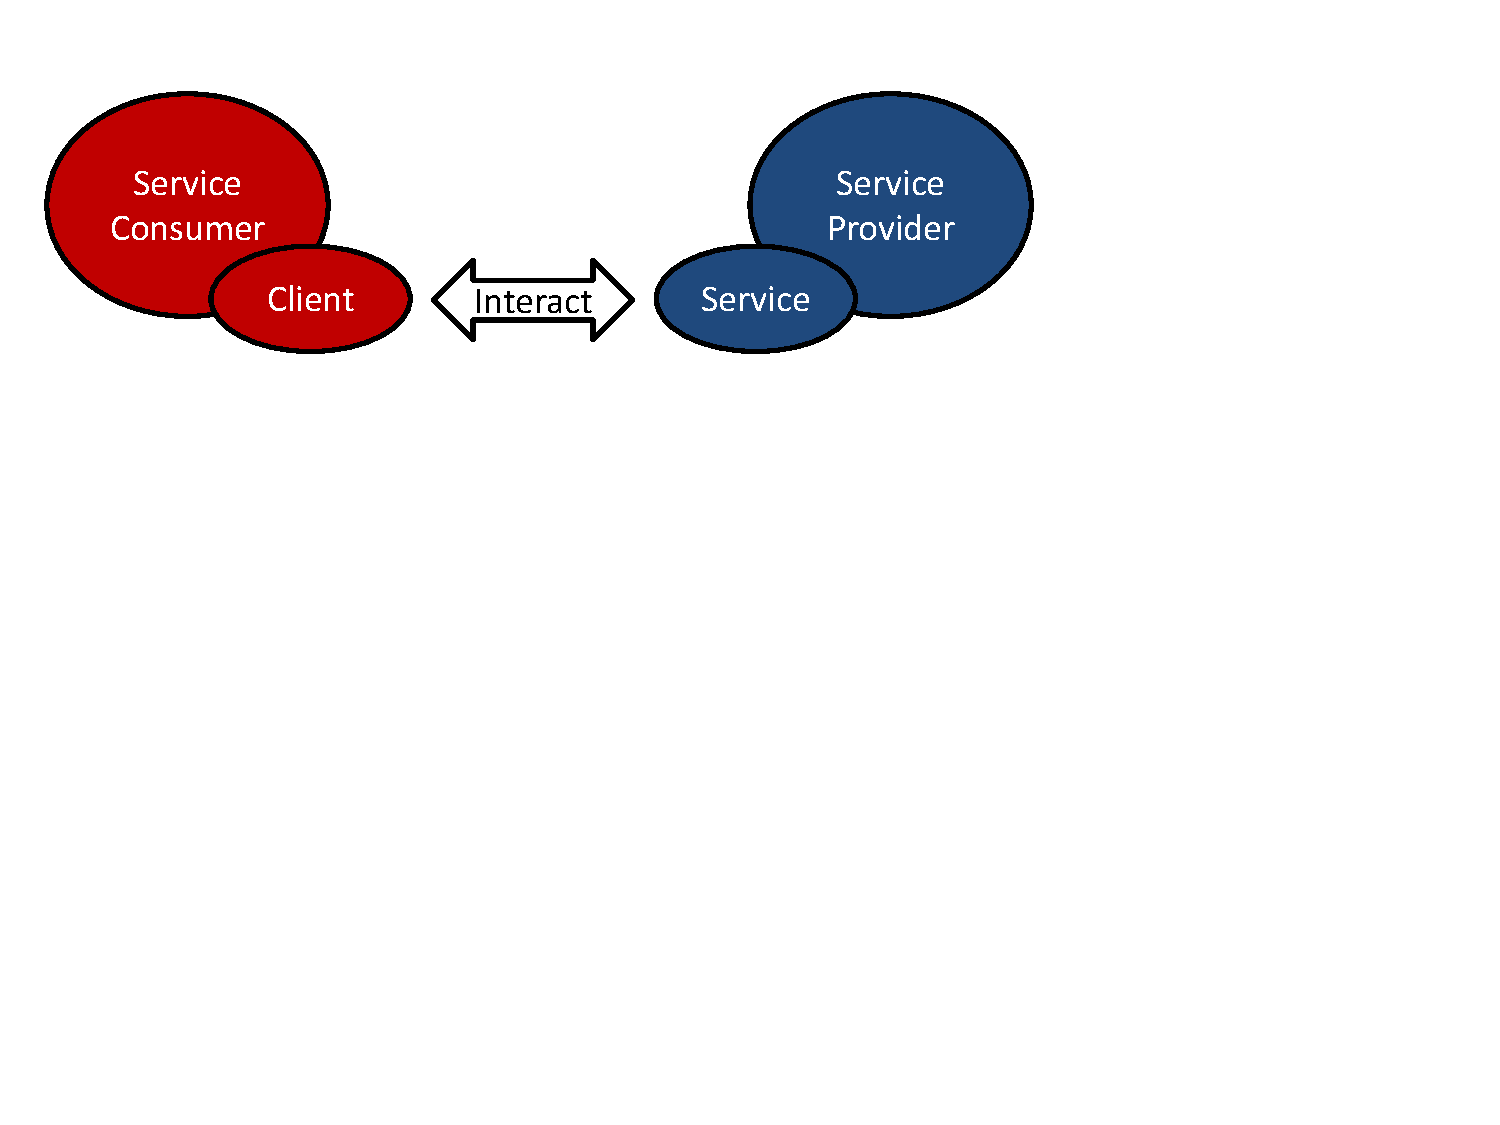
\includegraphics[width=0.8\textwidth]{Bilder/soa.pdf}}
	\caption{Service Oriented Architecture}
	\label{fig:soa}
\end{figure}

A very important design principle with respect to mashups and mashup composer tools is the ``Service
Composability'' principle, which encourages the design of services in a loosely coupled manner and
hence can be reused in multiple solutions that are themselves made up of composed services \cite{soa}.

\section{Related Work}

The approach, which is discussed in this thesis, is not the only one, which can be applied to
realize the discussed scenario (see Section \ref{sec:scenario}). Hence, the most interesting
approaches with respect to this thesis will be summarized subsequently.

\subsection{A Service-Oriented Approach to Document-Centric Situational Collaboration Processes}
This paper \cite{schuster2009} introduces a service-oriented approach to integrate enterprise
documents within SOA landscapes. Therefore, it represents documents as compositions of stateless
software services, which can be described, published, discovered, selected and accessed - with
respect to the SOA paradigm. Furthermore, these services can communicate based on an event-based
communication model and interact according to specified document interaction patterns.\newline The
composition of the available document services, like content, transformation, composition or layout
services, finally takes place in a mashup infrastructure, like the ones that are provided by IBM
Mashup Center, Microsoft Popfly or Yahoo Pipes.

\subsection{FAST}
The main objective of the \textit{``FAST (Fast and Advanced Storyboard Tools)''} project \cite{fast}
is to create a new visual programming environment that facilitates the development of complex
front-end gadgets, involving execution of relatively complex business processes that rely on back-end
semantic web services.\newline Instead of first building programs that orchestrate available
semantic web services and then trying to figure out how to implement interaction with the users at
given points of the process execution flow, programmers will start from the front-end gadgets that the user will see
and interact with, and then visually establish connections to back-end Web Services, going through
process execution flows if necessary.\newline
The goal of the project is to develop ``mashup-able'' gadgets that rely on semantic web services
independent of the mashup platform, which is used to display or further process the gadgets. That
means that the resulting gadgets should be deployable within all three of the inspected mashup tools or
platforms as they are called with respect to FAST. However, at the moment FAST only supports a
single target mashup platform, namely EzWeb \cite{ezweb}, which is still in beta state
\cite{fast_paper}.

\subsection{MarcoFlow}
MarcoFlow aims at going one step beyond state-of-the-art workflow management and service composition
and proposes an original model, language and running system for the composition of distributed UIs,
an approach that allows to easily bring together UIs, web services and people in a single
orchestration logic and tool. The type of applications that can be developed with MarcoFlow are
called ``distributed UI orchestrations'' \cite{marcoflow}.

However, MarcoFlow is more targeted at designing the workflow and orchestrating distributed web
services and UIs within an application which requires technical skills and a deep insight in the
workflow and the involved services. Whereas the goal of the mashup composers, like Microsoft Popfly,
Yahoo Pipes and IBM Mashup Center, and this thesis is the simple composition and adaptation of
applications on a user interface which can be handled by end-users without technical insight.

\subsection{Approaches based on the OSGi Framework}
The following two approaches extend the OSGi Framework with useful and interesting functionalities
to build a custom enterprise service bus or a multi-tier enterprise client/server application and
hence could have been used as basis for the Component Framework. However, none of the approaches is
dedicated towards visually designing applications and minimizing the required programming skills
and hence the most lightweight framework was chosen as basis.

\subsubsection{Swordfish}
Swordfish \cite{swordfish} provides an open source framework that allows application developers and
system integrators to build their own enterprise service bus (ESB), which enables the combination of
services in an easy and flexible manner. It is based on proven technologies like Apache ServiceMix
and hence on OSGi as well as on the JBI standard for messaging abstraction and message routing
between components.\newline Furthermore, the integrated Service Registry allows a loose coupling
between service providers and service consumers, which are connected dynamically at runtime. The
communication takes place directly between two services or components respectively and therefore
needs no intermediary which could become a performance bottleneck \cite{swordfish_whitepaper}.

\subsubsection{Riena}
The Riena platform \cite{riena} is a framework for building multi-tier enterprise
client/\newline server applications and therefore broadens the usage of the service oriented
architecture of OSGi by providing access to local and remote services in a transparent way.\newline Using the provided
concepts and programming model the enterprise application can be developed regardless of the target
location and the individual components can be either placed on the client or server side of
the application depending on the business requirements \cite{eclipse_riena}.\newline Furthermore,
Riena provides a redesign for the Eclipse RCP workbench which tries to simplify the navigation
within the created applications.

\subsection{Dashboards}
Related to this thesis are also dashboard applications. Stephen Fex defines a dashboard as follows
\cite{stephen_few}:

\msQuote{A dashboard is a visual display of the most important information needed to achieve one or
more objectives; consolidated and arranged on a single screen so the information can be monitored
at a glance.}

Hence, a dashboard is a software product aimed to integrate information from multiple components into
a unified display. For example, it might obtain information from the local operating system, from
applications that may be running, and from remote sites on the Web and present it as though it all
came from the same source.\newline As sophisticated dashboards can connect to nearly any data source
and are highly customizable, they are also used within enterprises to provide a dynamic read-out of
personalized, business-critical information.\newline Popular examples for dashboards which can be
used within business are the ``WebSphere Dashboard Framework''
\cite{websphere_dashboard} from IBM and the ``ARIS Performance Dashboard'' \cite{aris_dashboard}
from IDS Scheer.

Nevertheless, dashboards are not designed to let the simple information displays or widgets
communicate, exchange information or react to user inputs and hence are not applicable for the
described scenario (see Section \ref{sec:scenario}).

\subsection{Portals and Portlets}
Portals and Portlets provide a first approach to component-based UI development \cite{portlets}.
Portlets are full-fledged, pluggable Web application components which generate document markup
fragments (e.g., HTML) and can be arranged on a portal page. A portal server therefore allows users
to manage and customize such portal pages and furthermore provides single sign-on and role-based
personalization.

However, portals and portlets exhibit the same drawbacks as dashboards and hence are not applicable
as well.

\section{Research Objectives}
\label{sec:research_objectives}

Goal of this thesis is to investigate existing mashup composer tools, which are aimed at end-users
without any programming skills and provide a simple user interface for accessing and aggregating
different data sources and hence developing mashups and applications respectively. The conducted
evaluation of these tools and the adopted set of evaluation criteria should help identifying the
major lacks and missing functionality, which are required to realize a scenario like the one
introduced in Section \ref{sec:scenario}.

Hence, the major research objective is, besides the evaluation, the development of the
``Component Framework'' which tries to support the requirements of the introduced scenario. The
framework should be built on technologies which are standardized and well approved in practice,
since the target applications, which should be applicable in business as well, should be as stable,
fail-safe and secure as possible.

\section{Research Method}

As addressed in Section \ref{sec:research_objectives} the adopted research method is the evaluation
of existing mashup composer tools. Therefore, specific evaluation criteria which represent the
requirements for these tools to realize a scenario, like the one that is described in Section
\ref{sec:scenario}, are introduced, the evaluation is conducted and the final results are presented
and analyzed.

Having identified the problems which are discovered during the evaluation process and are not
solved by the existing tools, requirements for the implementation of a solution are derived.
These requirements form the basis for the prototype framework which tries to compensate the observed
limitations and is implemented as part of this thesis. Finally, to validate the feasibility of the
proposed framework a test application based on the air ambulance scenario has been developed.

\section{Structure of the Thesis}
The remainder of this thesis is structured as follows:

\textbf{Chapter \ref{chapter:evaluation}} evaluates three software products which are used to create and
design mashups. Each of them is targeted at the easy access and aggregation of data in order to
produce output that is more valuable than the separate data input streams.

\textbf{Chapter \ref{chapter:requirements}} discusses the evaluation results and formulates a set of
requirements for a software product which eliminates the weaknesses of the evaluated products and
provides means for realizing the scenario introduced in Section \ref{sec:scenario}.

\textbf{Chapter \ref{chapter:osgi}} introduces and illustrates the well-known OSGi Framework, which
provides the basis for the developed prototype framework, which is called ``Component Framework''. The
Component Framework is especially implemented for this master thesis and tries to support the
introduced requirements.

\textbf{Chapter \ref{chapter:applications}} introduces two applications which are based on the implemented
framework and therefore demonstrate the feasibility of the underlying concepts.

\textbf{Chapter \ref{chapter:summary}} concludes the thesis with a summary.
\chapter{Evaluation of Mashup Composers}
\label{chapter:evaluation}

This chapter deals with the evaluation of existing tools, which are used for composing and
designing mashups. First, the most important features of each tool are discussed before the tools
are evaluated against certain evaluation criteria. These criteria represent requirements for realizing the air
ambulance scenario (see Section \ref{sec:scenario}) or similar ones.

The evaluation process is based on \cite{Heinrich2000} and therefore starts with the evaluation
preparation.

\section{Evaluation Preparation}

The evaluation preparation section introduces the various evaluation objects
and defines the goals and criteria for the evaluation process.

\subsection{Evaluation Objects}
\label{sec:evaluation_objects}

The inspected evaluation objects are different software products for designing mashup components
without the need for writing any code. To select respective products an extensive search was
conducted to find information on mashups and mashup-composers. This search resulted in a list of
ten to fifteen tools which were shortlisted and from which Microsoft Popfly, Yahoo Pipes and IBM Mashup
Center were selected. These three tools are not only the most popular ones, but also the most
advanced. All of them are - at least as test version - available to the public. The fact that
big companies like Microsoft, Yahoo and IBM stand behind these tools provides further arguments for
the choice.

In the following the selected tools are introduced.

\subsubsection{Microsoft Popfly}
\label{sec:microsoft_popfly}

As stated on the official Popfly Website \cite{microsoft_popfly},

\msQuote{Microsoft Popfly is the fun, easy way to build and share mashups,
gadgets, games, web pages, and applications. Popfly consists of a set of online
visual tools for building web pages and mashups, and a social network of creators
where you can host, share, rate, comment and even remix creations from other
Popfly users.}

\par This statement shows that Microsoft Popfly is not only designed to create simple mashups, but also to set up web pages and games. Nevertheless, the main
focus of this work will lie on the mashup-feature of this tool.

Therefore, the next section introduces the ``Mashup Creator'', which provides an
interface for composing mashups. Figure
\ref{fig:microsoft_popfly_tool_architecture} gives an overview of the mashup structure and the
involved software products that are needed to compose mashups with Microsoft Popfly.

\begin{figure}
	\centering
	\fbox{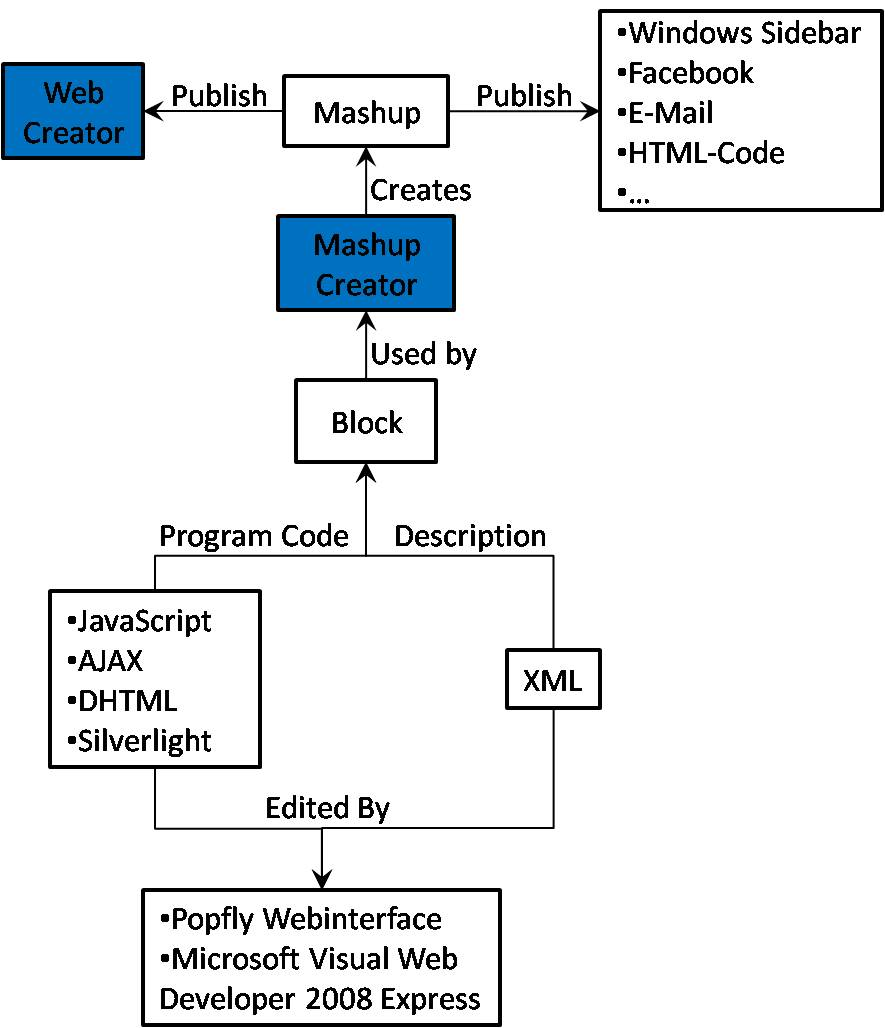
\includegraphics[width=0.8\textwidth]{Bilder/microsoft_popfly_tool_architecture.jpg}}
	\caption{Microsoft Popfly - Overview}
	\label{fig:microsoft_popfly_tool_architecture}
\end{figure}

\paragraph{Mashup Creator}

The Mashup Creator, like all other Popfly tools, is provided as web application and can therefore
be accessed via the Popfly website.

\begin{figure}
	\centering
	\fbox{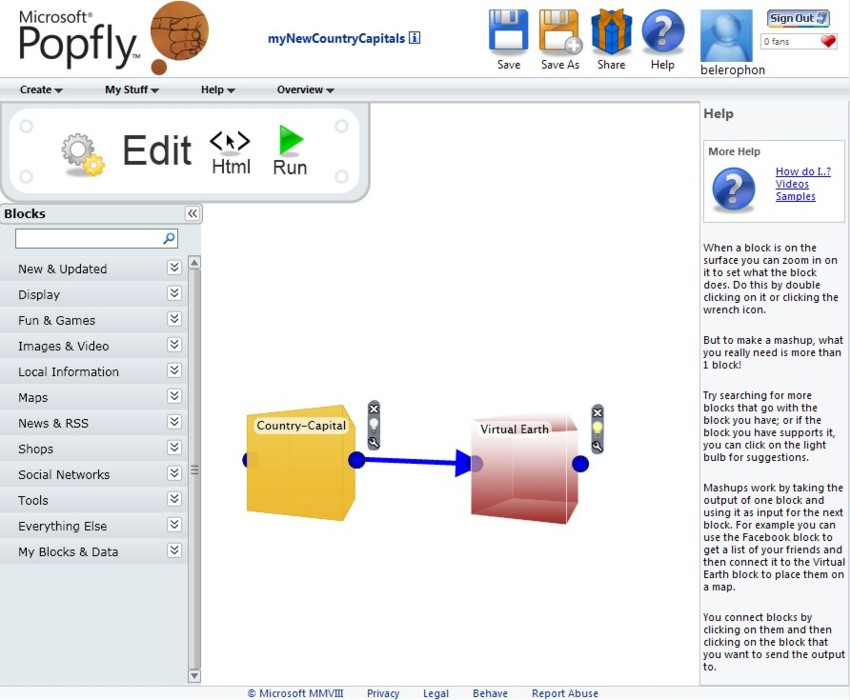
\includegraphics{Bilder/microsoft_popfly_mashup_creator.jpg}}
	\caption{Microsoft Popfly - Mashup Creator}
	\label{fig:microsoft_popfly_mashup_creator}
\end{figure}

To compose mashups, the tool provides a simple user interface with a working
area and a catalog of basic building units, which are called ``blocks''. These blocks consist of
two parts: One part contains the program code, which implements the functionality, the other one is an
XML-Metadata file, which describes the block and its functionality in a human readable form.

The program code of simple data access blocks is written in
JavaScript\footnote{JavaScript is an object-oriented scripting language, which
allows the development of enhanced user interfaces and websites.}, whereas more
complex presentation layer blocks like ``Virtual Earth'' are based on
AJAX\footnote{asynchronous JavaScript and XML}, DHTML\footnote{DHTML is a
collection of technologies like HTML and JavaScript used together.} or
Silverlight.

In order to extend the already large catalog of pre-built blocks and to enable
the building of new blocks or editing existing ones, Microsoft provides a simple
web-interface to edit the JavaScript code. In addition, Microsoft provides the ``Popfly
Explorer''-plug-in for the freely available ``Microsoft Visual Web Developer 2008 Express'' as an
alternative to create and edit more complex blocks.

The pre-built blocks are sufficient for creating simple mashups without having to implement custom
blocks.

Figure \ref{fig:microsoft_popfly_mashup_creator} shows the Mashup Composer with two interconnected
blocks.

\paragraph{Using the created Mashup}
As soon as the mashup creation process is finished the mashup can be saved, published to other
Popfly users, to the Windows sidebar, to a Facebook profile or to various other social networking sites and
integrated into websites. The integration into websites is also supported by the so-called ``Web
Creator'', which is a part of Microsoft Popfly and is used to design simple websites.

\paragraph{The concept of a Mashup within Microsoft Popfly}
Each Microsoft Popfly mashup comprises the following parts (remember the
structure of a mashup described in Section \ref{sec:mashup}):

\begin{enumerate}
\item Every mashup needs one or more of the various \textbf{data source}
blocks. This can be the Flickr photo database, some RSS-feed, a database of the
capitals of all countries, as well as many other kinds of data sources.\newline
Furthermore, Popfly provides blocks for user inputs, which enable, for example,
the specification of RSS-feed URLs at runtime.

\item The second essential part of a mashup is the \textbf{display}, which
presents the information, received from the data source blocks, in a suitable
form. Therefore, Popfly provides blocks like virtual earth, image slide-show
displays or simple tables with a few columns.

\item The third major part is the ability to \textbf{connect two blocks} in order
to exchange data and communicate respectively.\newline Naturally, most blocks
offer not only a single function that can be called and there can be
compatibility problems concerning the data that is transferred between the
blocks. Therefore, most blocks have to be edited slightly or additional blocks,
which convert and process the data, have to be introduced.\newline In the case of
Virtual Earth (see Figure \ref{fig:microsoft_popfly_edit_block}) the operation,
which processes the data of the data source block, can be chosen,
input-parameters for this operation can be specified and additional properties
can be defined (see Figure
\ref{fig:microsoft_popfly_concept_of_a_block}). As the Virtual Earth
block in the depicted example gets its data from the Country-Capital block, this
block is enabled as data source. If there is no compatible data source block
available, the input fields can be filled with custom values.
\end{enumerate}

\begin{figure}
	\centering
		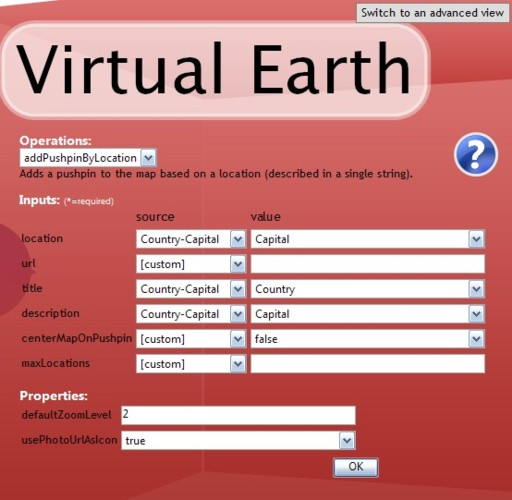
\includegraphics{Bilder/microsoft_popfly_edit_block.jpg}
	\caption{Microsoft Popfly - Editing the Virtual Earth block}
	\label{fig:microsoft_popfly_edit_block}
\end{figure}

\begin{figure}
	\centering
	\fbox{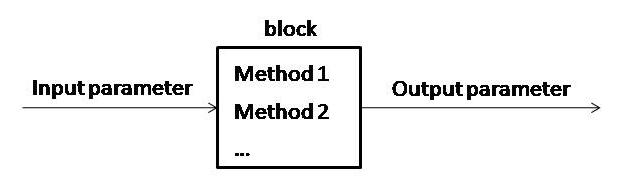
\includegraphics[width=0.8\textwidth]{Bilder/microsoft_popfly_block.jpg}}
	\caption{Microsoft Popfly - Structure of a block}
	\label{fig:microsoft_popfly_concept_of_a_block}
\end{figure}

The mashup depicted in Figure \ref{fig:microsoft_popfly_capitals} is one of the simplest mashups that
can be created and is based on the structure which is depicted in Figure
\ref{fig:microsoft_popfly_concept_of_a_simple_mashup}. Naturally most mashups do not only consist of
two building blocks, but are more complex. Therefore, Microsoft provides, for example, blocks to
combine or merge two or more data sources, to filter special data and to check if the data complies
with certain conditions to support various different application scenarios. For better
understandability Figure \ref{fig:microsoft_popfly_concept_of_a_complex_mashup} depicts the
structure of such a complex mashup.

\begin{figure}
	\centering
		\fbox{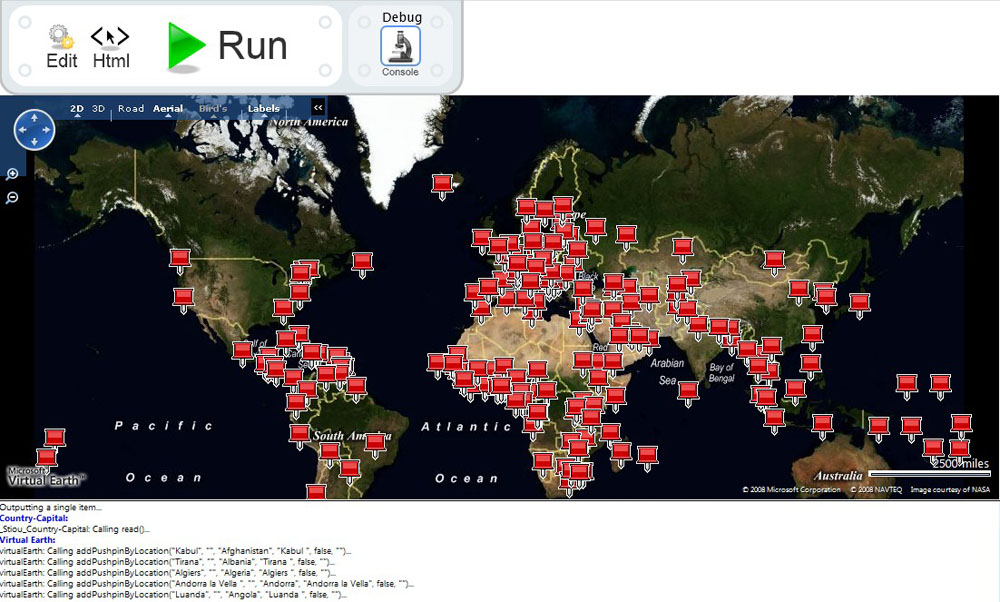
\includegraphics[width=0.8\textwidth]{Bilder/microsoft_popfly_capitals.jpg}}
	\caption{Microsoft Popfly - The ``Country Capitals'' Mashup in Action}
	\label{fig:microsoft_popfly_capitals}
\end{figure}

\begin{figure}
	\centering
	\fbox{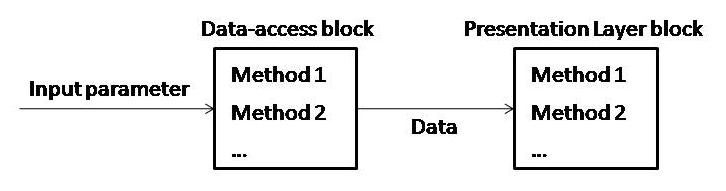
\includegraphics[width=0.8\textwidth]{Bilder/microsoft_popfly_simple_mashup.jpg}}
	\caption{Microsoft Popfly - Structure of a simple Mashup}
	\label{fig:microsoft_popfly_concept_of_a_simple_mashup}
\end{figure}

\begin{figure}
	\centering
	\fbox{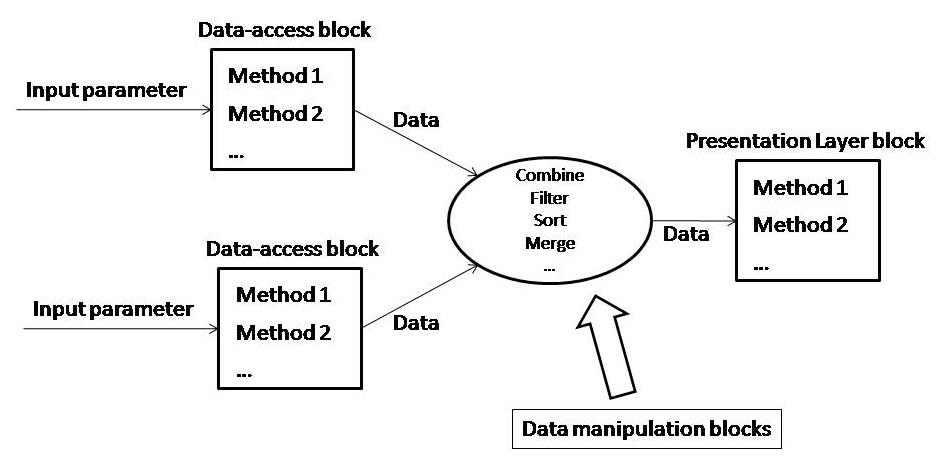
\includegraphics[width=0.8\textwidth]{Bilder/microsoft_popfly_complex_mashup.jpg}}
	\caption{Microsoft Popfly - Structure of a complex Mashup}
	\label{fig:microsoft_popfly_concept_of_a_complex_mashup}
\end{figure}

\paragraph{Mashup Execution}
To test and use the created mashup, Microsoft Popfly differentiates between build and execution
time. This means that the output of the composed mashup is only displayed when it is executed by
``running'' the mashup as it is called. The resulting mashup (see Figure
\ref{fig:microsoft_popfly_capitals}) is loaded within the Mashup Creator and a debug console can be
displayed to analyze possible errors. Switching between ``edit'' and ``run'' mode can be done
easily and hence allows a quick and smooth adaptation of the built mashup.

\subsubsection{Yahoo Pipes}
\label{sec:yahoo_pipes}

The second tool that is analyzed and tested is also a web application, is
developed by Yahoo and called ``Yahoo Pipes'' \cite{yahoo_pipes}. It allows the
creation and modification of pipes, as mashups are called within Yahoo Pipes, as
well as browsing through pipes designed by other individuals.

\paragraph{The Pipes Editor}
Similar to Microsoft Popfly, the pipes editor (see Figure
\ref{fig:yahoo_pipes_pipes_editor}) provides a list of building blocks which are
called ``modules'' and a working area. Important to mention here is that the
catalog of building blocks can not be extended, but the development team has to be contacted and
informed about missing features instead.

\begin{figure}
	\centering
		\fbox{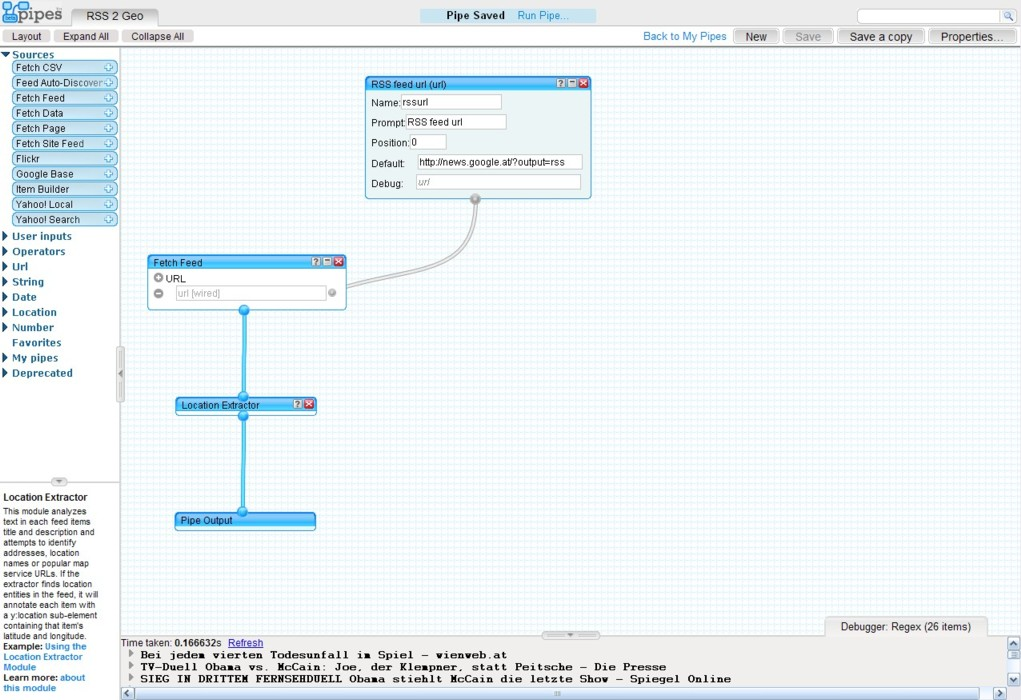
\includegraphics{Bilder/yahoo_pipes_pipes_editor.jpg}}
	\caption{Yahoo Pipes - The Pipes Editor}
	\label{fig:yahoo_pipes_pipes_editor}
\end{figure}

\paragraph{The concept of a Mashup within Yahoo Pipes}
The concept of a mashup within Yahoo Pipes is similar to Microsoft Popfly, but is realized slightly
differently.

\begin{enumerate}
  \item Again the first part of a mashup is constituted by a \textbf{data source} block. The provided
  blocks can fetch nearly every data that is available on the web, but lack the functionality of
  accessing local databases or files.\newline Just like Microsoft Popfly, the Pipes Editor provides
  modules for user inputs. Compared to Popfly, these modules are more sophisticated and can therefore
  interact with all other modules without exhibiting compatibility problems.
  \item Naturally, every pipe needs a \textbf{display} to expose the fetched data in a   human
  readable form, but Yahoo Pipes does not provide any module that is explicitly   responsible for
  displaying data. Yahoo Pipes handles this problem differently   and provides a module that is
  called ``Pipe Output'', which is the endpoint   of every mashup. This final module does nothing
  else than parsing the   received data for image and location information. If there is no such data
  available, the feed items are arranged in a list. As soon as there is some information about
  images, the feed items are presented as a slide-show. Finally, if there is   geographical data
  included, the items are displayed on a map (see Figure \ref{fig:yahoo_pipes_google_news}).
  \item The third and final part of every mashup is the possibility to \textbf{connect the modules}  
  and to exchange data and communicate via this connection or channel   respectively.
\end{enumerate}

A big advantage over Popfly is the debug console which is available in the Pipes Editor, displaying
the current output data and thereby alleviates the mashup developing process.
  
Again, this concept describes one of the simplest mashups. Naturally, Yahoo Pipes can integrate
multiple blocks between data source and pipe output modules. These blocks can be used to combine,
filter, merge, split and process the data. Figures \ref{fig:yahoo_pipes_simple_mashup} and
\ref{fig:yahoo_pipes_complex_mashup} display the concepts behind simple and complex mashups created
with Yahoo Pipes.

\begin{figure}
	\centering
		\fbox{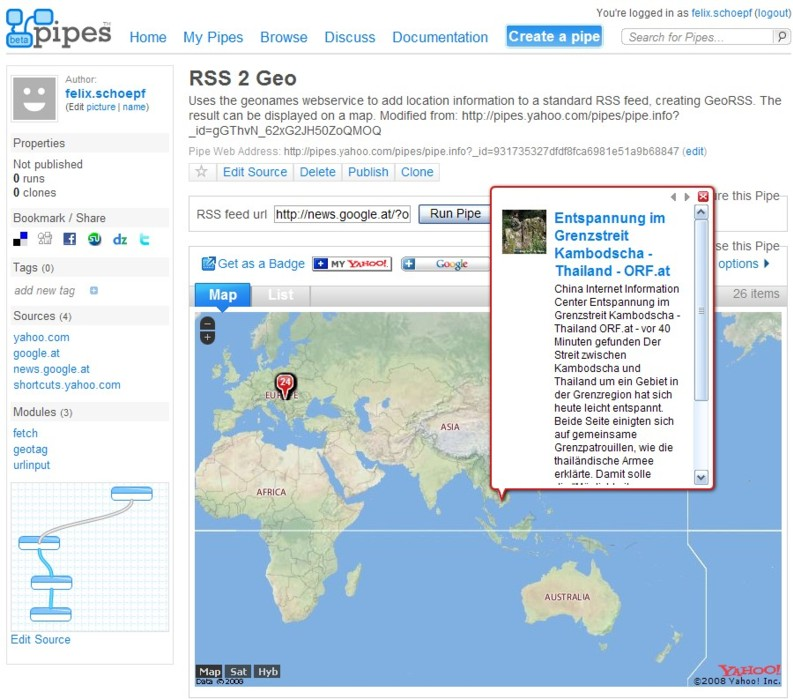
\includegraphics{Bilder/yahoo_pipes_google_news.jpg}}
	\caption{Yahoo Pipes - Running a pipe}
	\label{fig:yahoo_pipes_google_news}
\end{figure}

\begin{figure}
	\centering
		\fbox{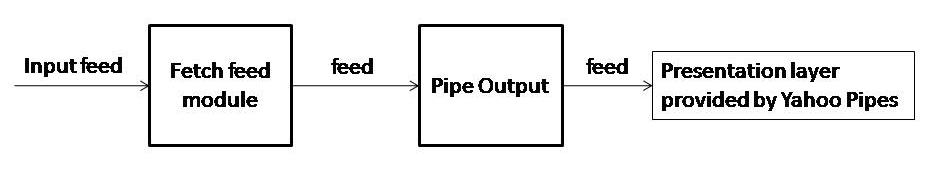
\includegraphics[width=0.8\textwidth]{Bilder/yahoo_pipes_simple_mashup.jpg}}
	\caption{Yahoo Pipes - Simple Mashup}
	\label{fig:yahoo_pipes_simple_mashup}
\end{figure}

\begin{figure}
	\centering
		\fbox{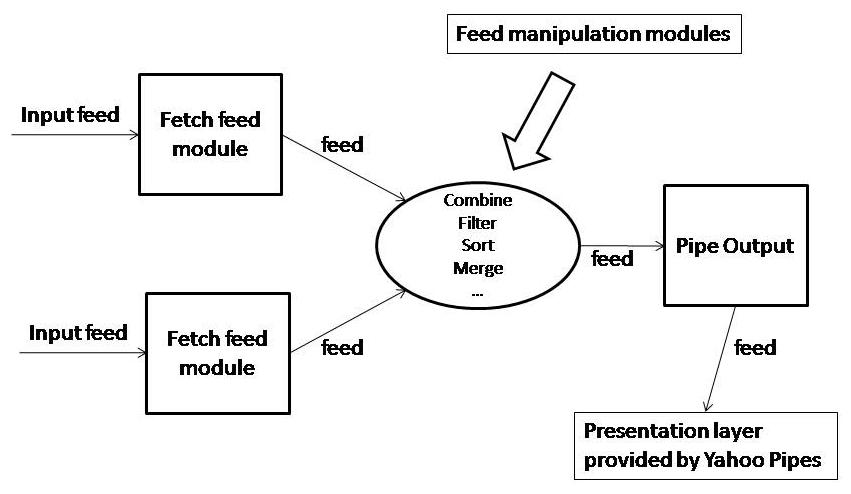
\includegraphics[width=0.8\textwidth]{Bilder/yahoo_pipes_complex_mashup.jpg}}
	\caption{Yahoo Pipes - Complex Mashup}
	\label{fig:yahoo_pipes_complex_mashup}
\end{figure}

\paragraph{Mashup Execution}
Similar to Microsoft, Yahoo makes a difference between build and runtime. As soon as a pipe is
``run'' a new browser window or tab opens and displays the output. Switching between the build and
runtime windows allows a quick adaptation of the current pipe.

\paragraph{Using the created Pipe}
Finally, if the development process is finished and the intended goals are
reached the pipe can be saved, published to other Yahoo Pipes users, to the
private Yahoo or Google page or to various social networking sites and
integrated into a website or a blog.

\subsubsection{IBM Mashup Center}
\label{sec:ibm_mashup_center}

Finally, the third tool to be tested is the ``IBM Mashup Center''
\cite{ibm_mashup_center}, which is focused on enterprise customers and
therefore resulted in a more complex application.

The Mashup Center mainly consists of two separate software products: ``InfoSphere MashupHub'' and ``Lotus
Mashups''. InfoSphere MashupHub is used for preparing all data sources and Louts Mashups is the
tool for composing the actual mashup (see Figure \ref{fig:ibm_mashup_center_concept}).

\begin{figure}
	\centering
		\fbox{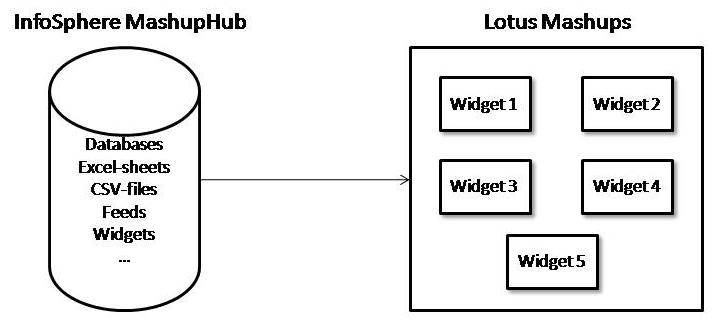
\includegraphics[width=0.8\textwidth]{Bilder/ibm_mashup_center_concept.jpg}}
	\caption{IBM Mashup Center - Concept}
	\label{fig:ibm_mashup_center_concept}
\end{figure}

\paragraph{InfoSphere MashupHub}
InfoSphere MashupHub is a lightweight information management environment where data sources
like databases, external web sources, Excel- or CSV-sheets are installed (see Figure
\ref{fig:ibm_mashup_center_mashuphub_all}). Visual tools for creating, storing, transforming and
remixing data easily and quickly can be included in the MashupHub \cite{ibm_mashup_center}.\newline
This means that data does not have to be refined within Lotus Mashups and the mashup composition
process respectively. This is a point where IBM Mashup Center differs from Microsoft Popfly and Yahoo
Pipes, where also the blocks for refining and editing the given data have to be placed on the working
area of the composition tool, which obviously limits the space for composing the actual mashup.

As soon as all necessary data sources are prepared within InfoSphere MashupHub
(see Figure \ref{fig:ibm_mashup_center_mashuphub_all}) they can be explicitly
added to Lotus Mashups to be available during the mashup composition process.

\begin{figure}
	\centering
		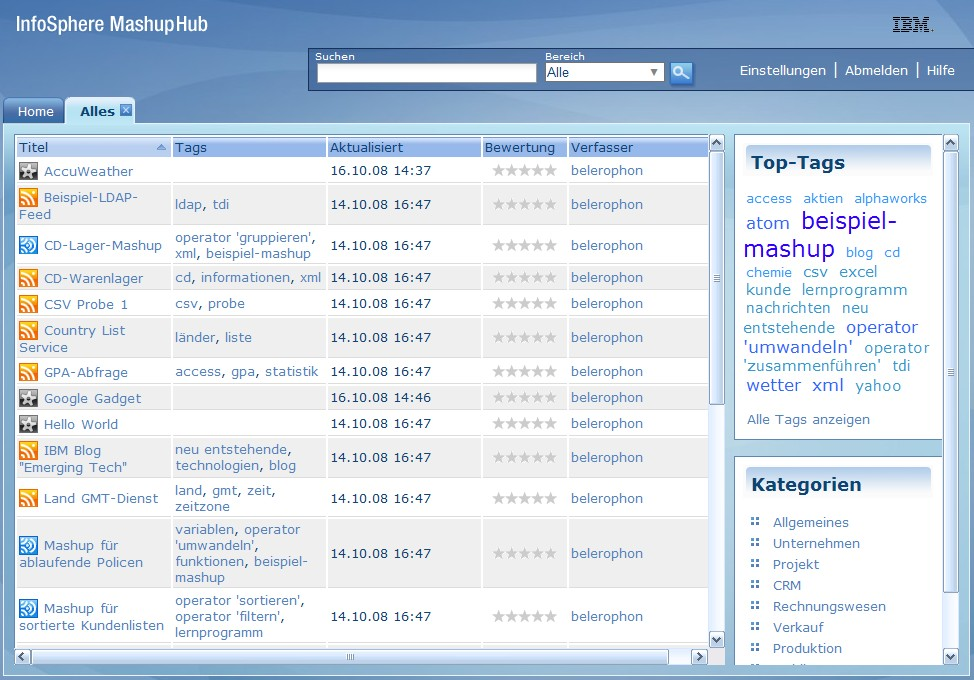
\includegraphics{Bilder/ibm_mashup_center_mashuphub_all.jpg}
	\caption{InfoSphere MashupHub - The Feeds, Widgets and Mashups}
	\label{fig:ibm_mashup_center_mashuphub_all}
\end{figure}

\paragraph{Lotus Mashups}
Lotus Mashups can have one or multiple sites, which are arranged in tabs. Furthermore, each site
provides a working area, where the building blocks can be placed on, has a name, can be deleted at
any time or made available for all other users of Lotus Mashups.

An additional search field can be used for finding components and data sources
respectively within InfoSphere MashupHub and thus adding them to the list of
available building blocks of Lotus Mashups.

\paragraph{The concept of a Mashup within IBM Mashup Center}
The base concept of Lotus Mashups are sites, where the widgets which display data can be arranged
(see Figure \ref{fig:ibm_mashup_center_mashups}). This means that the Mashup Center is more focused
on grouping widgets within sites and enabling data to be displayed in various forms on various sites
compared to the two other mashup composers.

Another big difference to Microsoft Popfly and Yahoo Pipes is the fact that
most mashups which were developed with these tools consist of only a single
widget within Lotus Mashups. This comes from the possibility of processing
data within Lotus Mashups and exposing the resulting data stream as widget.

But Lotus Mashups still provides the functionality to connect widgets, which
leads to the same structure than the other tools. Hence, a mashup consists of one or multiple
data source widgets, one or multiple data display widgets and connections between
them. Figure \ref{fig:ibm_mashup_center_mashups} depicts such a mashup: It
shows a data source widget, which displays customer data in a simple table and
is connected to three other widgets. One widget displays weather information
for the customers' address, another one displays the address on a map and the
third one shows the appropriate website.

Figure \ref{fig:ibm_mashup_center_mashup_concept} finally depicts the concept
behind such a mashup.

\begin{figure}
	\centering
		\fbox{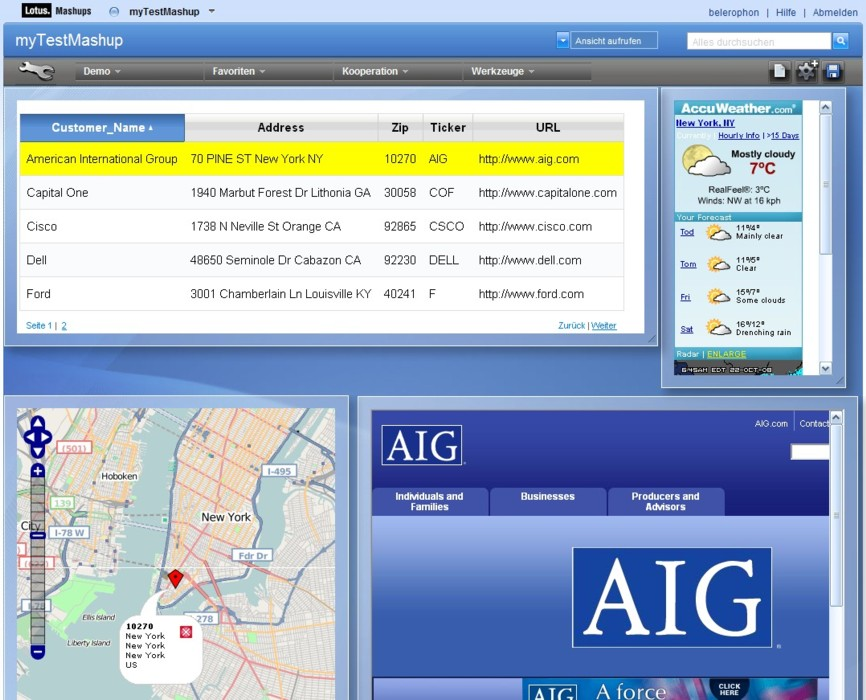
\includegraphics[width=0.8\textwidth]{Bilder/ibm_mashup_center_mashups.jpg}}
	\caption{Lotus Mashups - A sample Mashup}
	\label{fig:ibm_mashup_center_mashups}
\end{figure}


\begin{figure}
	\centering
		\fbox{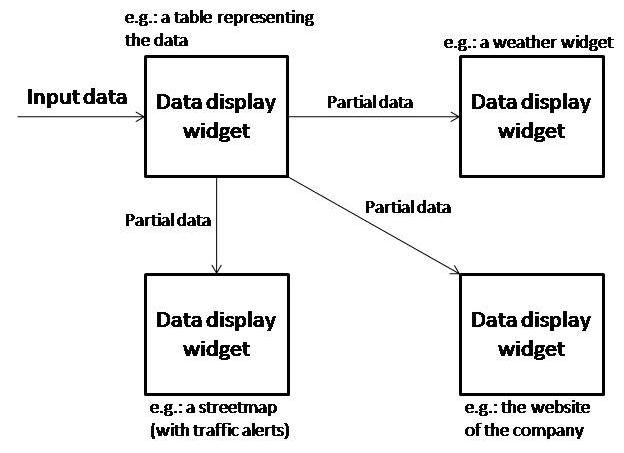
\includegraphics[width=0.7\textwidth]{Bilder/ibm_mashup_center_mashup_concept.jpg}}
	\caption{IBM Mashup Center - Mashup Concept}
	\label{fig:ibm_mashup_center_mashup_concept}
\end{figure}

\subsection{Evaluation Goal}

The goal of this evaluation is to obtain an impression of how powerful these mashup composers
are and how easy it is to develop small, but useful applications with them. Furthermore, the
evaluation should detect problems, which have to be solved, and missing features, which are
required to realize the discussed scenario (see Section \ref{sec:scenario}). Therefore, the next section introduces the
selected evaluation criteria.

\subsection{Evaluation Criteria}
\label{sec:evaluation_criterions}

\begin{itemize}
	\item \textbf{User Interface and Usability}\newline
	This part of the evaluation takes a closer look at the design and construction of the user
	interface. The user interface should be tailored towards end-users without programming experience
	and provide intuitive functionality to get quickly started.
	\item \textbf{Data Access and Processing}\newline
	The main goal of mashups is the processing of data from various data sources and thereby
	producing output data which is of value for the mashup consumer. Hence, every mashup
	composer has to provide building blocks which enable the access of various different data sources
	and furthermore provide blocks to combine, merge and process the received data. From this it
	follows that each tool also has to provide the functionality of exchanging data between
	blocks.
	\item \textbf{Extensibility}\newline
	This criterion takes a closer look at the possibility to extend the mashup composer with custom
	blocks to add special functionality and to adapt the mashup to the users' personal interests.
	\item \textbf{Multiple Instances}\newline
	Every mashup composer should be able to run multiple instances of the same component within a
	single mashup. This functionality is important for data access blocks, to fetch multiple
	data streams of the same format as well as for data processing and display blocks which are
	responsible for monitoring some kind of information, like the status of multiple flights (cf.
	Section \ref{sec:scenario}).
	\item \textbf{Grouping of Blocks}\newline
	As soon as a mashup gets more complex and multiple different data sets have to be displayed, the
	space provided by a single browser window is often too small. Therefore, the mashup composer tool
	should provide the functionality to group building blocks on different sites, which can be
	switched quickly.\newline Furthermore, two data sets that consist of multiple building blocks --
	like the monitor of an airplane (see Section \ref{sec:scenario}) -- have often to be compared.
	Hence, the tool should provide a feature to visually group the building blocks of one data set on the working area, to alleviate
	the comparison and to make the difference between the data sets more obvious.
	\item \textbf{Reusability of Groups}\newline
	This criterion deals with the reusability of grouped building blocks. Once a group is designed it
	should be able to save and reuse it either within the same or a different mashup. That means
	that a monitoring group for a single airplane (see Section \ref{sec:scenario}) can be saved and
	reused for a second airplane, by simply adapting the data source. The various groups can then
	be placed either on the same site or on different ones according to the use case.
	\item \textbf{Hot Deployment and Life-cycle Management}\newline
	This criterion addresses examples where created applications or mashups respectively should be
	adapted quickly without the need to restart the entire application.\newline Imagine the example
	from Section \ref{sec:scenario}, where the manager wants to monitor a changing number of
	airplanes over time. At the moment, the inspected mashup composers aren't flexible enough to
	display multiple groups of blocks on a single user interface or to add and remove a group or a
	monitored airplane respectively at runtime. However, for examples like this, it is necessary to
	enable the hot deployment of components which monitor an additional airplane as well as the
	functionality to stop a component and dispose it from the display as soon as the flight is over,
	without having to stop the monitoring process of other airplanes. From this it follows that the
	implemented components also require a life-cycle management within the running application.
	\item \textbf{Event Management}\newline
	This evaluation criterion deals with the provided possibilities of informing
	other blocks about events that occurred, without sending big amounts of data.
	That means that all interested blocks can register as event handlers for each
	specific event and hence can react to it, by, for example, updating the data source or
	opening an information window.\newline This mechanism can reduce
	the amount of data that is transferred and the coupling between blocks.\newline In connection with
	the air ambulance example (see Section \ref{sec:scenario}) the event management enables
	the propagation of technical problems concerning the airplane, information of the closedown of the
	destination airport and all the other events that can occur.
	\item \textbf{Logging}\newline
	The last criterion deals with the logging mechanism, which is needed for the logging of errors,
	warnings and other useful information. The acquired data can be used to analyze problems which
	occurred during the mashup creation and execution process and to apply data mining methods, which
	enable, for example, the analysis of user behavior.
\end{itemize}

\subsection{Rating}

In order to provide an overall assessment the inspected tools have been rated. For this purpose,
every mashup composer is awarded for each evaluation criterion (see Table
\ref{tab:TheEvaluationCriterions}) by either a ``+'', for fulfilling the respective criterion, or a
``o'' for the implementation of a partial solution or a ``-'' if the inspected criterion is missing.

\begin{table*}[h]
	\centering
		\begin{tabular}{|l|}
			\hline
				\textbf{Evaluation Criteria}\\
				\hline\hline
				User Interface and Usability\\
				\hline
				Data Access and Processing\\
				\hline
				Extensibility\\
				\hline
				Multiple Instances\\
				\hline
				Grouping of Blocks\\
				\hline
				Reusability of Groups\\
				\hline
				Hot Deployment and Life-cycle Management\\
				\hline
				Event Management\\
				\hline
				Logging\\
			\hline
		\end{tabular}
	\caption{Evaluation Criteria}
	\label{tab:TheEvaluationCriterions}
\end{table*}

\section{The Evaluation}

This section deals with the evaluation of the introduced mashup composers against the selected
evaluation criteria.
 
\subsection{User Interface and Usability}

Usability and the ease of use is one of the main goals of mashups. To enable the creation of simple
mashups by end-users, a clearly arranged, well structured and easy to use user interface is
indispensable.

\subsubsection{Microsoft Popfly}

For this purpose Microsoft Popfly groups its user interface into three main parts: A list of
available building blocks, which are categorized depending on their usage, a working area and a
help section. In addition, there are menu bars to edit the HTML-code, which surrounds the mashup,
to run the mashup as well as to save and share it.\newline Simple drag and drop enables the placing
of building blocks on the working area and the connection of these blocks. An additional interface
enables the adaptation of the input and output parameters of each block, which is necessary to
make them communicate and exchange data correctly.

\subsubsection{Yahoo Pipes}

Yahoo Pipes offers a user interface that looks quite similar to the one of Microsoft Popfly and
mainly consists of a list of building blocks and a working area. Furthermore, it provides detailed
information about each building block and a debugger console. This console displays the output of
the building block which is selected on the working area and hence constitutes a useful feature for
complex mashups. Again drag and drop is the way of creating pipes and connecting the single
building blocks.\newline Additional menu bars and buttons offer possibilities to create a new pipe,
save the current one, edit the properties of the mashup or execute it.

\subsubsection{IBM Mashup Center}

As IBM Mashup Center consists of two tools (i.e., Lotus Mashups and InfoSphere MashupHub) and is
designed for building sites containing various kinds of widgets, it is structured a little
differently.\newline Lotus Mashups -- the tool for designing the site -- provides a list of widgets
and a working area. Additional buttons enable the saving of the site and to browse the so-called
catalog, which is nothing else than a connection to the InfoSphere MashupHub, which constitutes the
repository for all widgets that can be used within Lotus Mashups.\newline As drag and drop is the
standard instrument to enable an easy and intuitive handling of applications it is also applied
within Lotus Mashups and enables the arrangement of the different widgets. The connection of the
widgets is not implemented by drawing visible arrows between the widgets, as with the two other
tools, but by specifying the target or source widget in a drop-down-list, which is provided by every
widget.

\subsubsection{Conclusion}

To sum up, all evaluated tools offer a well structured user interface, which is
easy and quite intuitive to use and enables the creation of a simple mashup within minutes.

The evaluation of the User Interface and Usability criterion hence leads to a balanced
result (cf. Table \ref{tab:RatingUserInterfaceAndUsability}).

\begin{table*}[h]
	\centering
		\begin{tabular}{|c|c|c|}
			\hline
				\textbf{Microsoft Popfly} & \textbf{Yahoo Pipes} & \textbf{IBM Mashup Center}\\
				\hline\hline
				+ & + & +\\
			\hline
		\end{tabular}
	\caption{Rating - User Interface and Usability}
	\label{tab:RatingUserInterfaceAndUsability}
\end{table*}

\subsection{Data Access and Processing}
\label{sec:data_access_and_aggregation}

This section evaluates the possibility of accessing and processing data with mashup composer tools.

\subsubsection{Microsoft Popfly}
Microsoft Popfly can access many data sources as long as they are published in the form of RSS feeds
or provide the data as character separated values. Furthermore, the catalog contains blocks to access
the Flickr database of photos or to get information from social networks like Digg or
Facebook. However, Popfly is limited to access data that is available on the web via simple
messaging standards. Local databases or data containers like Excel sheets remain unaccessible as long
as no custom block is implemented that provides this features.

To enable data processing Popfly provides blocks to combine data streams and to filter and sort
them. Unfortunately, no appropriate possibility to convert data from one format to another is
provided. This leads to data incompatibilities and constrains the communication between
blocks.\newline This problem leads to a limited number of blocks which can interact as long as no
custom blocks are implemented, which do the necessary conversion.

\subsubsection{Yahoo Pipes}
As Yahoo Pipes is designed to process feed data, it can fetch all kinds of RSS or Atom feeds which
are available on the web. Furthermore, it can access data which is available in CSV, XML or JSON
format as well as Yahoo search results and data from the Google merchant center, which constitutes
a database for products. Unfortunately, Yahoo Pipes also lacks the possibility to access
local databases or data containers like Excel and it is limited to data sets which are available or
can be converted to the RSS format.

For the purpose of processing data, Yahoo Pipes provides effective support. The data which is
fetched by the various modules is transformed to a RSS feed which can then be combined with other
feeds, filtered, sorted or split. For special processing the data can be sent to an external web
service which implements the necessary data transformation operations, which are not available
within Yahoo Pipes yet.

\subsubsection{IBM Mashup Center}
IBM Mashup Center allows the access of web feeds as well as of databases, Excel sheets, Access data
files and web services and hence provides more extensive data access means than the other two mashup
composers.

In the context of data processing IBM has to deal with the same problems as the other evaluated
tools. The provided building blocks for combining, filtering, extracting and transforming data, are
applicable for most of the pre-built blocks, but still there exist incompatible target blocks.
Hence, the user must implement sophisticated data transformation blocks to enable the communication
between all pre-built and custom blocks.

\subsubsection{Conclusion}

As none of the tools can completely fulfill the ``Data Access and Processing'' criterion, but
provide partial solutions, they are all rated with ``o'' (cf. Table
\ref{tab:RatingDataAccessAndAggregation}). Furthermore, it is important to mention that there will
exist data incompatibilities and hence data processing errors or problems, as long as mashup
composers do not make any restrictions on the used data format. Another solution for this problem is
the possibility of extending the tools with custom data transformation blocks and therewith placing
the responsibility for making a required data format compatible on the end-user.

\begin{table*}[h]
	\centering
		\begin{tabular}{|c|c|c|}
			\hline
				 \textbf{Microsoft Popfly} & \textbf{Yahoo Pipes} & \textbf{IBM Mashup Center}\\
				\hline\hline
				o & o & o\\
			\hline
		\end{tabular}
	\caption{Rating - Data Access and Processing}
	\label{tab:RatingDataAccessAndAggregation}
\end{table*}

\subsection{Extensibility}

The possibility to extend the available catalog of building blocks with custom blocks is an
important feature for each of the inspected tools and hence is evaluated in this section.

To fulfill this criterion Microsoft Popfly provides two mechanisms to develop custom blocks. Either
an existing block is edited or a new block is implemented by using the Visual Web Developer 2008
Express Edition. Also IBM Mashup Center can be extended by using an available software product,
namely the IBM Lotus Widget Factory. Yahoo Pipes, unfortunately, does not provide any possibilities
to extend its catalog of building blocks.

Table \ref{tab:Extensibility} displays the evaluation result for the ``Extensibility'' criterion.

\begin{table*}[h]
	\centering
		\begin{tabular}{|c|c|c|}
			\hline
				\textbf{Microsoft Popfly} & \textbf{Yahoo Pipes} & \textbf{IBM Mashup Center}\\
				\hline\hline
				+ & - & +\\
			\hline
		\end{tabular}
	\caption{Rating - Extensibility}
	\label{tab:Extensibility}
\end{table*}

\subsection{Multiple Instances}
\label{sec:multiple_instances}

Every mashup composer should provide an infrastructure that enables the execution of multiple
instances of the same building block in parallel. This is also a very important requirement for the
air ambulance example (see Section \ref{sec:scenario}) which has to display multiple airplanes at
the same time. It would be very impractical to have to implement a custom block for each airplane.
Hence, it should be possible to add multiple identical ``airplane components'' at the same time and
adapt the information they hold, by providing, for example, the flight number.

This criterion is fully realized by IBM Mashup Center and only partially by Microsoft Popfly and
Yahoo Pipes. These two tools limit the possibility to use multiple components, which are responsible
for displaying data, at the same time. That means that data source and processing components, which
are responsible for fetching and aggregating or converting data are handled differently than
display components.

Table \ref{tab:RatingMultipleInstances} holds the result for the ``Multiple Instances'' criterion.

\begin{table*}[h]
	\centering
		\begin{tabular}{|c|c|c|}
			\hline
				\textbf{Microsoft Popfly} & \textbf{Yahoo Pipes} & \textbf{IBM Mashup Center}\\
				\hline\hline
				o & o & +\\
			\hline
		\end{tabular}
	\caption{Rating - Multiple Instances}
	\label{tab:RatingMultipleInstances}
\end{table*}

\subsection{Grouping of Blocks}

The ``Grouping of Blocks'' criterion is neither realized by Microsoft Popfly nor by Yahoo Pipes
and only partially by the IBM Mashup Center. Indeed, IBM provides the possibility to group blocks
and widgets respectively within so-called ``sites'', which can be switched easily, but lacks the
feature of grouping blocks within a single site.

Therefore, Yahoo Pipes and Microsoft Popfly are awarded with a ``-'' and IBM Mashup Center with a
``o'' (cf. Table \ref{tab:RatingGroupingOfBlocks}).

\begin{table*}[h]
	\centering
		\begin{tabular}{|c|c|c|}
			\hline
				 \textbf{Microsoft Popfly} & \textbf{Yahoo Pipes} & \textbf{IBM Mashup Center}\\
				\hline\hline
				- & - & o\\
			\hline
		\end{tabular}
	\caption{Rating - Grouping of Blocks}
	\label{tab:RatingGroupingOfBlocks}
\end{table*}

\subsection{Reusability of Groups / Hot Deployment and Life-cycle Management / Event Management /
Logging}

As Microsoft Popfly and Yahoo Pipes lack the functionality of grouping blocks they also cannot
provide a mechanism to reuse groups and hence cannot score in the context of the ``Reusability of
Groups'' criterion. Unfortunately, also IBM Mashup Center fails to support the possibility to reuse
the created ``sites'' within other mashups.

Furthermore, each of the three tools differentiates between development and execution time. Hence,
none of the mashup composers supports hot deployment of additional components or provides life-cycle
support for components or building blocks respectively.

Although each of the evaluated tools provides the possibility to directly connect multiple building
blocks and to send data via these channels, none of them enables the more lightweight
publish-subscribe event mechanism (see Section \ref{sec:communication}).\newline Naturally the
direct connections can be misused for sending events, but this does not change the fact that the direct connections were introduced to
exchange data sets and require a tighter coupling than the event mechanism, which exchanges only
small pieces of information.

Finally, the evaluated mashup composers also miss a logging mechanism, which hence leads to the
evaluation results which are listed in Section \ref{sec:overall_evaluation_results}.

\subsection{Overall Evaluation Results}
\label{sec:overall_evaluation_results}

Table \ref{tab:RatingsTableWithoutWeightingFactors} shows the overall evaluation results concerning
the ratings each mashup tool was awarded with.

\begin{table*}[h]
	\centering
		\begin{tabular}{|c|c|c|c|c|c|c|c|c|c|}
			\hline
				\textbf{Evaluation Object} & 
				\begin{sideways}\textbf{User Interface and Usability}\end{sideways} &
				\begin{sideways}\textbf{Data Access and Processing}\end{sideways} &
                \begin{sideways}\textbf{Extensibility}\end{sideways} &
                \begin{sideways}\textbf{Multiple Instances}\end{sideways} &
                \begin{sideways}\textbf{Grouping of Blocks}\end{sideways} &
                \begin{sideways}\textbf{Reusability of Groups}\end{sideways} &
                \begin{sideways}\textbf{Hot Deployment and Life-cycle Management}\end{sideways} &
				\begin{sideways}\textbf{Event Management}\end{sideways} &
                \begin{sideways}\textbf{Logging}\end{sideways}\\
                \hline Microsoft Popfly 	& + & o & + & o & - & - & - & - & -\\
                \hline Yahoo Pipes 			& + & o & - & o & - & - & - & - & -\\
                \hline IBM Mashup Center 	& + & o & + & + & o & - & - & - & -\\
			\hline
		\end{tabular}
	\caption{Overall Ratings}
	\label{tab:RatingsTableWithoutWeightingFactors}
\end{table*}
\chapter{Requirements}
\label{chapter:requirements}

This section analyzes the strengths and weaknesses of the mashup composer tools which could be
identified during the evaluation process and hence formulates the requirements for a software
product which eliminates the weaknesses and provides means for realizing the introduced scenario
(see Section \ref{sec:scenario}).

\begin{itemize}
  \item \textbf{Requirement 1: Simple User Interface}\newline The user interface that is provided by
  the evaluated tools can be mostly handled with the mouse and supports convenient drag and drop
  functionality. Hence, it does not need an extensive documentation and simple mashups can be designed
  very quickly by end-users.\newline Since user interfaces are one of the strengths of the mashup
  composers, they should be adopted and extended with the missing functionality, like grouping of
  blocks (cf. Requirement 5).
  \item \textbf{Requirement 2: Data Access and Processing}\newline As mashups and applications
  respectively most likely require data from local databases or from the web it is necessary to
  enable the access of a wide variety of data sources (from simple comma separated files
  over databases, over web services to live status information from an airplane).\newline In order
  to process the data which is received by the data access blocks it is necessary that each block can
  send data to and receive data from every other block. This enables the implementation of data
  conversion, aggregation and filtering components (cf. Requirement 3: Extensibility), which prepare
  the data for further receiving blocks and therewith reduce data incompatibilities between
  different building blocks.
  \item \textbf{Requirement 3: Extensibility}\newline The inspected mashup composers provide useful
  pre-built building blocks, but they are still not sufficient to cover every scenario, mashup or
  application respectively. Hence, the catalog of building blocks has to be extensible to provide
  displays for every kind of data and data access or processing functions for unfamiliar data
  formats.\newline Although creating a block requires programming skills, the process of
  implementing custom blocks should be as easy as possible and supported very well.
  \item \textbf{Requirement 4: Running multiple Instances of a Block}\newline This requirement
  is necessary to, for example, monitor multiple airplanes in parallel (see Section
  \ref{sec:scenario}), where the same building block is required multiple times. As IBM Mashup
  Center handles this problem quite well, this functionality should be adopted within the
  implementation of the solution.
  \item \textbf{Requirement 5: Grouping of Blocks}\newline This is one of the requirements which is
  not fulfilled to its full extend by any of the inspected tools, but constitutes a major requirement
  to fulfill the air ambulance scenario (e.g., when multiple flights have to be monitored at
  the same time).\newline Grouping of blocks should be enabled either in the form of multiple
  groups of components on a single user interface or in the form of multiple user interfaces, which are
  easily switchable.\newline This leads to a better solution for the air ambulance scenario.
  Having the grouping functionality, every block which displays information about the flight --
  like a map with the current position of the airplane or a table which provides information about
  crew and passengers -- can be arranged within a single group. In this way the information is
  encapsulated and the different flights can be distinguished more easily.
  \item \textbf{Requirement 6: Reusability of Groups}\newline The possibility of reusing groups is
  the next major requirement to realize the air ambulance scenario and to alleviate the process of
  developing more complex applications. Let us take the airplane monitor application which is
  responsible for displaying real-time information about multiple airplanes in parallel. The
  monitor of a single airplane consists of multiple different blocks and thus forms a group.
  Without the ability to reuse a group the blocks would have to be rearranged for each
  airplane.\newline Hence, applications which fulfill this requirement enable the saving of groups
  and thus also the arrangement of whole groups on the working area. As a consequence, groups can be
  handled like single building blocks and can be added to and removed from the mashup or application
  respectively by using simple drag and drop mechanisms.
  \item \textbf{Requirement 7: Hot Deployment and Life-cycle Management}\newline None of the
  evaluated tools support hot deployment and life-cycle management and hence are not applicable for the
  discussed scenario (see Section \ref{sec:scenario}).\newline The problem is, that once a mashup is
  designed, executed and used it cannot be adapted to user or role specific needs. Therefore, a
  framework is needed which supports the starting and stopping of components and groups at runtime
  as well as the installation of absolutely new components within the framework. The different
  states of a component, like installed, started and stopped must be handled by a life-cycle
  management system, which furthermore enables the hot deployment of components.
  \item \textbf{Requirement 8: Event Management}\newline As soon as a mashup becomes more complex
  and a considerable amount of data is involved, effective event handling needs to be in place.
  Imagine a data source block which has to send the whole data to each of the various interested
  data display blocks as soon as only a single data entry is updated.\newline A better solution for
  realizing this scenario would be to send an event as soon as the data is updated and if a display
  block is interested in the new data, it can poll the data from the data source block.
  Furthermore, the event management system can be extensively used to provide interested blocks
  with information about all kinds of events, like, for example, technical problems of an airplane.
  Therefore, it should be possible to declare blocks as event publishers as well as event handlers
  or listeners respectively.\newline As a consequence, each block has to provide human readable
  information about which events it can send to enable the receiver to react correctly.
  \item \textbf{Requirement 9: Logging}\newline As long as the programmers of software
  products cannot guarantee that their implementation is error-free, the integration of a logging mechanism is
  very helpful to get information about the errors that happened. This functionality should be
  integrated into every pre-built block as well as in the custom-built ones.\newline Furthermore, the
  logging mechanism can be used to conduct data and process mining methods.
\end{itemize}
\chapter{Component Framework}
\label{chapter:osgi}

To address the requirements described in Chapter \ref{chapter:requirements}, the ``Component
Framework'' has been developed as part of this master thesis. As the underlying technical basis the
OSGi Framework is used.

Section \ref{sec:osgi} therefore introduces the ``OSGi Service Platform'', which forms the basis for
the Component Framework and is specified by the ``OSGi Alliance'' \cite{osgi-alliance}. The OSGi
Alliance is a worldwide consortium of technology innovators, which assures interoperability of
applications and services based on the OSGi Service Platform.

% Implementations of the OSGi Service Platform therefore provide means to install bundles, services and
% additional functionality respectively at runtime. That means that a running application, which is
% based on this platform, can be extended with further functionality, without restarting it.

Having the necessary background information, Section \ref{sec:component_framework} finally describes
the developed ``Component Framework'' in detail. It explains the functionality that was obtained by
the OSGi Service Platform as well as the extensions or adaptations that were implemented to realize the
requirements introduced in Section \ref{chapter:requirements}, like extensibility, running multiple
instances of a block, grouping of blocks, reusability of groups, event management and logging.

\section{OSGi Service Platform}
\label{sec:osgi}

This section introduces the OSGi Service Platform which has been used as underlying technical basis
for the development of the Component Framework.

The ``OSGi Service Platform'' is a dynamic module system for Java that allows the dynamic integration
and remote management of bundles (i.e., a cohesive unit of classes and resources) and services.
Furthermore, the service platform offers means to install, start, stop and uninstall bundles and
services at runtime without stopping and restarting the platform as a whole.\newline The
specification of the OSGi Service Platform is publicly available and can be accessed via the website
of the OSGi Alliance \cite{osgi-alliance}. The current version of the specification is 4.1 and
consists of three major parts, namely the ``Core Specification'', the ``Service Compendium and the
``Mobile Specification''.

\noindent\textbf{\textit{Core Specification:}}\newline The Core Specification
defines the OSGi Framework and Framework Services which are based on it. The OSGi
Framework is the base component of the Service Platform and provides the
infrastructure for installing, starting, stopping and uninstalling bundles and
services.

\noindent\textbf{\textit{Service Compendium:}}\newline The Service Compendium
includes a series of standard services, which are built on top of the OSGi
Framework and provide special functionality for various use cases. Examples of
standard services are a logging or configuration service as well as an event
service, which provides an interface for handling events throughout the
framework.

These services can be loaded at system startup or installed at runtime and are
registered at the service registry, where they can be accessed by every bundle
and service throughout the whole framework.

\noindent\textbf{\textit{Mobile Specification:}}\newline The Mobile Specification
includes a subset of the services, which are specified by the Service Compendium,
and adds some special services for mobile devices, which are also built on top of
the core specification.

\subsection{OSGi Framework}
\label{label_osgi_framework}
The cornerstone of the OSGi service platform is the ``OSGi Framework'' which
constitutes a container for bundles and services.

A \textbf{bundle} is a cohesive unit of classes and resources which can be
installed and uninstalled in the framework. These classes and resources are not
visible to other bundles initially. In order to make them visible and therefore
usable for other bundles, the packages containing the classes and resources, have
to be exported explicitly. Similarly, bundles which want to use the exported
packages have to import these. This mechanism enables a loose coupling between
the various bundles.\newline As soon as a bundle is installed in the OSGi
Framework, it tries to resolve the dependencies and to allocate the needed
packages respectively. If the required packages are not available in the system,
the bundle can not be started.

Another means of decoupling and service orientation is the ability of bundles to
use \textbf{services}. These services are Java-objects which are registered with
their interface-names at the so-called ``Service Registry''. This service
registry is available throughout the whole framework. Therefore, other bundles
can query the registry and obtain a service for further usage. No information
about the implementation or about the bundle that exposes the service is needed.

Finally, the \textbf{Management Agent}, which is part of the OSGi Framework,
enables the administration of bundles. In a very basic form this management agent
provides a text-based console which offers possibilities to install, uninstall,
start and stop bundles at runtime.

\subsection{OSGi Framework Specification}
The specification of the OSGi Framework is subdivided into multiple logic layers
(see Figure \ref{fig:osgi_framework_logic_layers}):

\begin{figure}
	\centering
		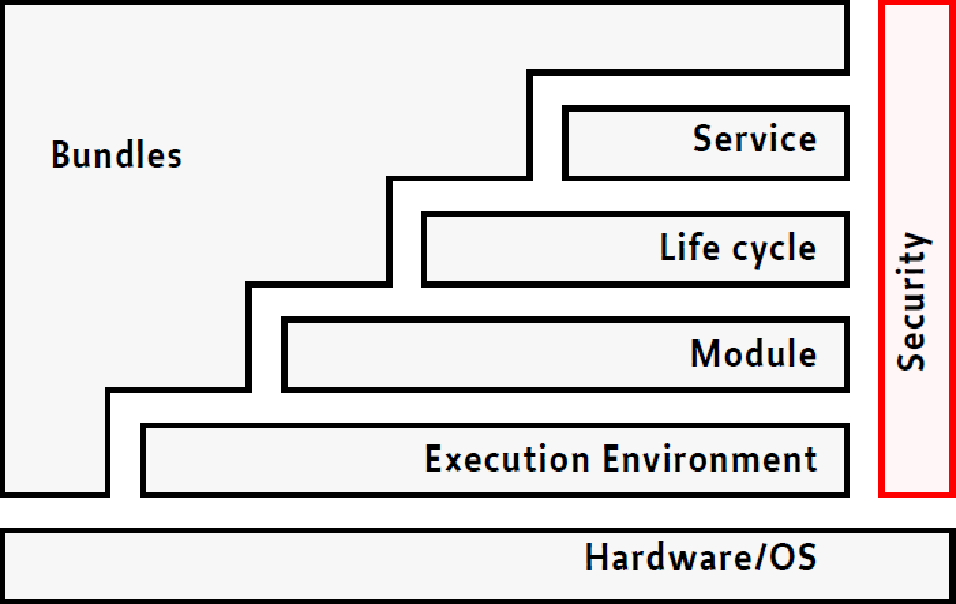
\includegraphics[width=0.8\textwidth]{Bilder/osgi-framework.pdf}
	\caption{OSGi Framework - Logic Layers}
	\label{fig:osgi_framework_logic_layers}
\end{figure}

\subsubsection{Execution Environment}
The OSGi Framework is specified in a way that enables the execution on various
Java-platforms. Therefore so-called ``Execution Environments'' are defined. These
execution environments are representations of concrete Java-runtimes, which
constitute the needed classes, interfaces and methods.

Two execution environments are specified in the Service Compendium:
\begin{itemize}
  \item The \textbf{OSGi/Minimum-1.1} defines the minimal environment that is needed for the
  execution of the OSGi Framework and the general services.
  \item A superset of the OSGi/Minimum-1.1 execution environment is the
  \textbf{CDC-1.0/Foundation-1.0}, which is a derivation of the JME Foundation Profile
  \cite{jme_foundation_profile}.
\end{itemize}

Based on the given premises concerning hardware, processing power and memory
resources the adequate execution environment has to be chosen.

But not only the OSGi Framework itself specifies the execution environment it
needs, also single bundles can specify a special execution environment. If such
a bundle is to be installed in the OSGi Framework it is checked if the given
execution environment satisfies the bundle's specification. If this is the case
the bundle is installed.

\subsubsection{Module-Layer:} \label{paragraph_module_layer} The module-layer
defines the bundle as the basic modularization-unit within the OSGi Service Platform. Technically, a bundle is
nothing else than a Java-archive, which contains the classes and resources for
the implementation of the functionality that should be provided by this
bundle.\newline Additionally, a bundle includes a ``Manifest''-file (see Figure
\ref{fig:manifest}), which contains various information about the bundle,
described in a declarative way. This information is needed by the framework to
run the bundle correctly.\newline The symbolic name and the version information,
for example, are needed to explicitly identify a bundle within the OSGi Service
Platform.\newline Also the dependencies between bundles, described in Section
\ref{label_osgi_framework}, are defined in the Manifest-file.

\begin{figure}
	\centering
		\fbox{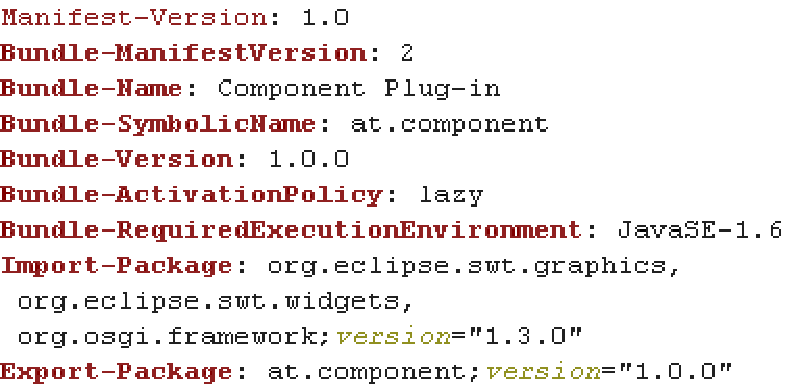
\includegraphics[width=0.8\textwidth]{Bilder/manifest.pdf}}
	\caption{MANIFEST.MF example}
	\label{fig:manifest}
\end{figure}

\subsubsection{Life-Cycle-Layer:}
\label{label_life_cycle_layer}
While the module layer describes the static aspects of bundles, the
life-cycle-layer specifies the dynamic ones.\newline
It defines the various states (see Figure \ref{fig:life_cycle_states}) a bundle
can have and the conditions and actions, which can lead to a state-change. In order to manipulate
the states of a bundle a so-called ``Management Agent'' implements an interface to the OSGi
Framework, which allows to control the framework from the outside.
Therefore, a Management Agent can provide a simple console for firing commands or a more
complex user interface, which provides various administrator tools.\newline
The installation of a bundle is one of the four basic operations a
management agent supports. If a bundle is installed successfully in the framework it is in the
``INSTALLED'' state. As soon as the framework has resolved all
package-dependencies it moves to the ``RESOLVED'' state.\newline
As a second operation the management agent implements the functionality to
start a bundle, which leads to the ``ACTIVE'' state on success or to the
``RESOLVED'' state otherwise. The stop-operation leads to the ``STOPPING''
state and to the ``RESOLVED'' state as soon as the stopping-operation is
finished.\newline
Finally the fourth operation enables the uninstalling of the bundle, which
requires a ``INSTALLED'' or ``RESOLVED'' state. If the bundle is in ``ACTIVE''
state the stop-operation has to be called at first.\newline
In addition to the four basic operations the framework provides the
possibility to update or refresh a bundle, which provides the opportunity to
exchange a bundle with a different version of the same bundle.


\begin{figure}
	\centering
		\fbox{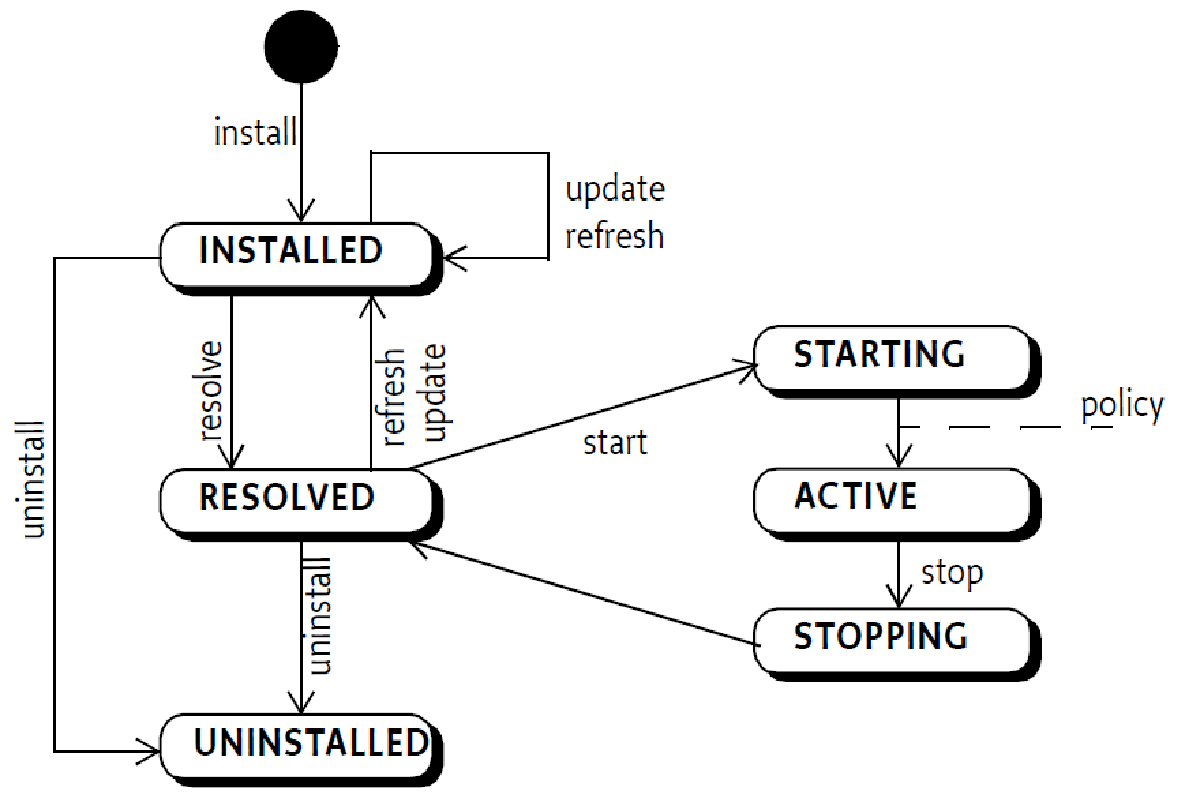
\includegraphics[width=0.8\textwidth]{Bilder/bundle-states.pdf}}
	\caption{Life-Cycle-States}
	\label{fig:life_cycle_states}
\end{figure}

\subsubsection{Service-Layer:}
\label{sec:service_layer}
The Service-Layer specifies a general Service-Model which makes services
available throughout the OSGi Framework. This model is implemented via a ``service
registry'', which constitutes the central point for registering, querying and
unregistering services.

As described in Section \ref{label_osgi_framework}, a ``Service'' is a simple
Java-object, which is registered at the service registry via it's interface-name.
Bundles that want to use this service can query the registration via the
interface-name and use the service. These bundles are called ``service consumers''
and do not know anything about the implementation details of a service. A
further detail that should be mentioned here is the possibility of having
multiple services implementing the same interface. Hence, the service consumer faces the
choice of using either one of the multiple services or all of them in parallel.

As services within the OSGi Framework can be registered and unregistered at any
time, a service consumer also has to anticipate the absence of a service and
provide sufficient error handling functionality. In order to alleviate the
handling of the described situations, the OSGi specification describes
possibilities like the``Service Tracker'', which provides means for detecting,
accessing and finally using registered services for a given service interface
name and wraps the complexity of directly using the service registry. 

The standard way of providing services is to set up one bundle that includes the
interface for a service and a second bundle that provides the implementation of
the interface and the service respectively. This scheme reduces dependencies and
allows the exchange of the service implementation at runtime.

A bundle that implements a new service and registers it at the service registry
is therefore called ``service producer''.

\subsubsection{Security Layer:}
The security layer is based on the Java 2 security architecture and provides
means for constraining execution rights for every single bundle. The support
for this security concept within an OSGi implementation is optional.

\subsection{OSGi Standard Services}
\label{sec:standard_services}
Based on the OSGi Framework Specification the OSGi Service Platform Service
Compendium and the OSGi Service Platform Mobile Specification define a series
of Standard Services, which provide solutions for various problems.\newline
The following service descriptions are only an excerpt of the full
specification and include only the services which can be associated with the
implemented application (see Section \ref{sec:component_framework}).

\noindent\textbf{\textit{Event Admin Service:}} The Event Admin Service
provides a mechanism for propagating events between bundles throughout the whole
framework. As an event can be identified by it's unique ``Topic'' every bundle
can specify an ``Event Handler'' for each of these topics.

\noindent\textbf{\textit{Wire Admin Service:}} In order to connect two services
at runtime the Wire Admin Service is needed. Each service can take the role of
an information consumer and/or producer and can exchange data via the
established connection.

\noindent\textbf{\textit{Application Admin Service:}} The Application Admin
Service empowers the OSGi Framework to manage external applications. Via the so
called Application Admin these applications can be for example started and
stopped.

\noindent\textbf{\textit{Log Service:}} The Log-Service specification implements
services for writing log-information like warnings, errors or debug-information.

\noindent\textbf{\textit{Configuration Admin Service:}} If services have to be
configured at runtime, the Configuration Admin Service is considered the best.

\noindent\textbf{\textit{Metatype Service:}} This service provides means for
adding meta-information to services, which can be queried and interpreted at
runtime. In connection with the Configuration Admin Service a ``Management Agent''
can use this information to provide a user interface for the configuration of a
service.

\noindent\textbf{\textit{Preference Service:}} The Preference Service implements the access to a
simple, hierarchic database, where bundles can store and read system- and user information.

\noindent\textbf{\textit{User Admin Service:}} This service specifies the
authorization and authentication of users, based on user- and group information.
Therefore, bundles can check if a specific user can access a certain
functionality.

\noindent\textbf{\textit{Declarative Service:}} With the help of this service a
bundle can declaratively define components with it's service-dependencies. The
so-called ``Service Component Runtime'' manages these components and dependencies
at runtime. Therefore a bundle does not have to manage the required services
anymore.

\subsection{OSGi Implementations}
\label{sec:osgi_implementations}

Several OSGi implementations are available and are therefore introduced in the following sections.

\subsubsection{Open Source Implementations}

\begin{itemize}
	\item\textbf{Eclipse Equinox}\newline Eclipse Equinox founds the basis for all Eclipse-applications
	and the Eclipse-IDE itself. Therefore Equinox is the commonly used OSGi Platform on the desktop.
	\item\textbf{Prosyst mBedded Server Equinox Edition}\newline This implementation of the OSGi
	Platform is available since March 2007, is based on Eclipse Equinox and provides, among others,
	additional standard services. Meanwhile Prosyst joined the Eclipse Foundation and is actively
	involved in the development of Equinox.
	\item\textbf{Knopflerfish}\newline Knopflerfish is developed by ``Makewave'' and provides an
	implementation of the OSGi-R4-specification.
	\item\textbf{Apache Felix}\newline Since 2007 Felix is one of the top-level-projects of Apache.
	Felix is based on the older OSGi implementation, called ``Oscar'' and is licensed under the
	``Apache License 2.0''.
\end{itemize}

\subsubsection{Commercial Implementations}

\begin{itemize}
	\item\textbf{Knopflerfish Pro}\newline Knopflerfish Pro is the commercial variant of Knopflerfish
	and extends the open source implementation with various drivers for GPS-devices and the serial
	COM-interface.
	\item\textbf{Prosyst mBedded Server Professional Edition}\newline Besides the open-source version
	Prosyst also provides the commercial mBedded Server Professional Edition. It is especially
	optimized toward performance and memory requirements. Therefore, it is qualified for platforms with
	very limited resources.
\end{itemize}


\section{Component Framework}
\label{sec:component_framework}

This section describes the ``Component Framework'', which has been implemented as part of this
master thesis and constitutes a proof-of-concept implementation. The framework is based on Java and
the described OSGi Service Platform and realizes the requirements introduced in Section
\ref{chapter:requirements}. Therefore, it provides an infrastructure or framework for developing,
managing, displaying and connecting so-called components. A component is the basic building block of
the Component Framework and is introduced in the next section.

\subsection{Components - The major Building Blocks of the Component Framework}
\label{sec:component}

A component within the Component Framework can be compared to blocks within the mashup composer
tools.

In more technical words a component is nothing else than a service which is implemented and
registered by an OSGi bundle (see Section \ref{label_osgi_framework}). In order to make the
component service seamlessly integrable into and manageable by the Component Framework it has to
implement a predefined service interface.

As soon as the service is registered at the service registry it is accessible throughout the entire
framework and the necessary methods to display the component user interface within an application
can be invoked. Moreover, the Component Framework enables the distinction between ``normal''
components and more complex components, which can have ``child-components'' allowing the grouping
of components (see Section \ref{sec:project}).

Summing up, a component is an application with a user interface, which is managed and displayed by
the Component Framework.

\subsection{Grouping of Components (Requirements 5 and 6)}

As one of the major requirements for the Component Framework was Requirement 5 ``Grouping of
Blocks'' (see Section \ref{chapter:requirements}), this section introduces the various grouping
methods which are included in the Component Framework.

The grouping of blocks requirement describes two different methods. The concept of ``projects''
realizes the first method which is responsible for displaying multiple user interfaces, which are
easily switchable and the concept of ``complex components'' realizes the second method and hence
provides means to display multiple groups of components on a single user interface.

\subsubsection{Projects - Containers for Components}
\label{sec:project}
To realize the requirement of multiple user interfaces, which are easily switchable, the concept of
``projects'' was introduced. For this purpose, a hierarchical structure was implemented, which means
that each component has a parent component and possibly one or multiple child components. The only
component that has no parent is the so-called project-component, which is the top-level component of
a project. As the Component Framework's intention is to enable the simple composition of
applications, the definition of projects and the introduction of a component hierarchy extend the
framework with the functionality of editing multiple projects or applications respectively in
parallel and grouping components on multiple sites according to their logical connection.

Furthermore, the Component Framework enables the saving and deploying of projects, which fulfills
Requirement 6 ``Reusability of Groups''.

\subsubsection{Complex Components}
\label{sec:complex_components}
The requirement of displaying multiple groups of components on a single user interface was realized
by introducing so-called ``complex components''. As described previously the Component Framework
introduces a parent child relationship between components. A complex component therefore is a
component which can have multiple child components and can be used as a top-level component for the
project (see Section \ref{sec:project}). The ``Group'' and ``Tabfolder'' components which were
implemented for the prototype application are examples for such components.

Figure \ref{fig:project_structure} finally depicts the overall structure of a project, which can be
compared to the well-known ``composite pattern'' \cite{GammaHelmEtAl95}.

\begin{figure}
	\centering
		\fbox{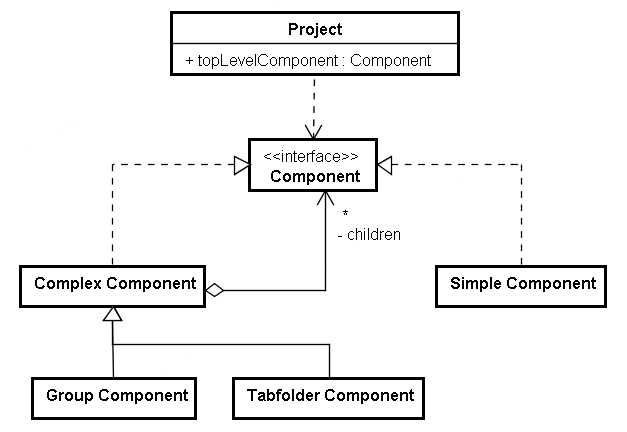
\includegraphics[width=0.98\textwidth]{Bilder/project-diagram.png}}
	\caption{Component Framework - Structure of a Project}
	\label{fig:project_structure}
\end{figure}

Figure \ref{fig:framework_ui} shows the realization of the project within the prototype
application. The red rectangle shows the project-component, the blue rectangle enframes the
so-called ``Group'' component (see Section \ref{sec:complex_components}), which can have multiple
child components and every green rectangle constitutes a simple component.

\begin{figure}
	\centering
		\fbox{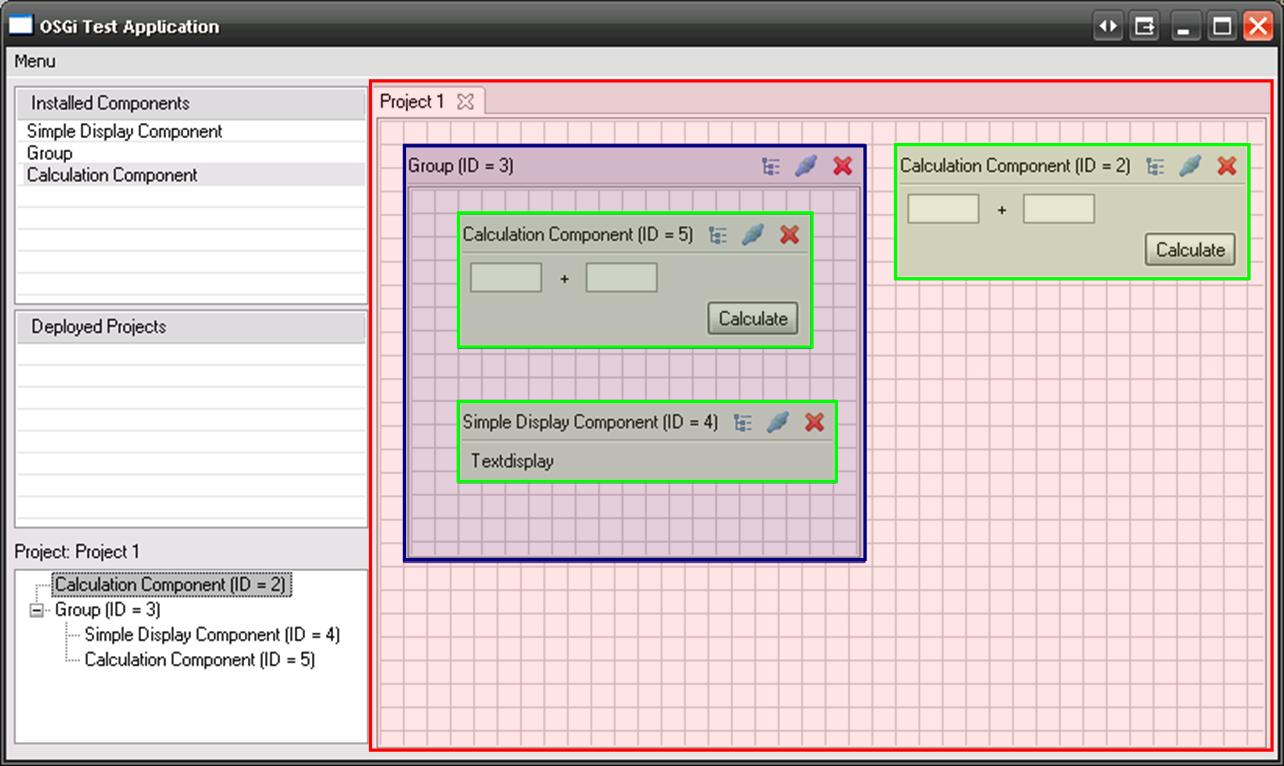
\includegraphics[width=1.2\textwidth,
		angle=90]{Bilder/framework_ui.jpg}}
	\caption{Component Framework - User Interface}
	\label{fig:framework_ui}
\end{figure}

\paragraph{Group Component}
The group component provides a working area where child components can be dropped and arranged
within a grid. Furthermore, it attaches a menu bar to each child component and provides
possibilities to drag and drop child components to other group components and to resize and rename every child component. The
items within the menu bar furthermore enable the configuration of connections to other components
(see Section \ref{sec:wire_admin}), the display of information about events which are
published by the child component (see Section \ref{sec:event_admin}) and the stopping
of the component.\newline
The goal of implementing such a component was to provide a work-area similar to those of the
inspected mashup tools (cf. Requirement 1 ``Simple User Interface'').

Figure \ref{fig:group_component} depicts a group component with a single child component, which
again is a group component.

\begin{figure}
	\centering
		\fbox{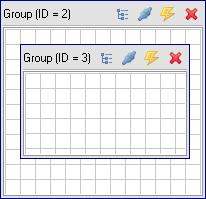
\includegraphics{Bilder/group_component.jpg}}
	\caption{The Group Component}
	\label{fig:group_component}
\end{figure}

\paragraph{Tabfolder Component}
The tabfolder component provides, as the name implies, a tabfolder which can hold multiple child
components as tabitems. Again, the child components can be added by simply dropping them from the
catalog into the tabfolder. The component also provides a menu bar which provides methods for
renaming the currently selected child component as well as connecting it to other components (see
Section \ref{sec:wire_admin}).

Figure \ref{fig:tabfolder_component} depicts a tabfolder component with two child components,
namely a group and a tabfolder component.

\begin{figure}
	\centering
		\fbox{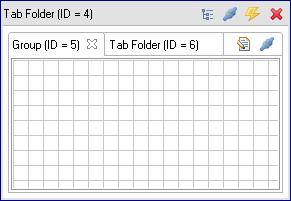
\includegraphics{Bilder/tabfolder_component.jpg}}
	\caption{The Tabfolder Component}
	\label{fig:tabfolder_component}
\end{figure}

As the working area and the tabfolder container are provided by single components and the Component
Framework is extensible (see Section \ref{sec:extensibility}) it is quite easy to either customize
the existing complex components and therewith create an individual working area or to extend the
framework with new components, which, for example, provide a user interface for dropping components
into a table or menu bar (cf. Requirement 3 ``Extensibility'').

\subsection{Services of the Component Framework}

This section describes the services which were implemented for the Component Framework to realize
Requirement 2 ``Data Access and Processing'', Requirement 4 ``Running multiple Instances of a
Block'', Requirement 7 ``Hot Deployment and Life-cycle Management'', Requirement 8 ``Event
Management'' and Requirement 9 ``Logging''.

The services of the Component Framework include the Component Starter Service, which is responsible
for starting multiple instances of a component, a simple ID service, which provides a unique ID
within a project of the Component Framework, extensions for the Wire Admin and Event Admin services
which enable data exchange and communication between components, and the powerful Component Service
which is responsible for managing the life-cycle of simple and complex components as well as
projects.

\subsubsection{Introduction: The OSGi Framework as Basis for the Component Framework}
The basis of the Component Framework is formed by the implementation of the OSGi Framework provided
by Eclipse, called ``Equinox''. This framework integrates the functionality to install, start, stop
and uninstall bundles that implement a component at runtime as well as to register services at the
service registry. Thereby, the OSGi Framework provides a good basis to fulfill Requirement 4
``Running multiple Instances of a Block'' and Requirement 7 ``Hot Deployment and Life-cycle
Management''.

Furthermore, Eclipse Equinox integrates multiple services which are contained in the OSGi Standard
Services specification (see Section \ref{sec:standard_services}) and provide the functionality to
communicate and exchange data between services and components respectively and are hence adapted for
the usage with components within the Component Framework.

\subsubsection{Component Starter and ID Service (Requirement 4)}
\label{sec:component_starter_service}
One of the major requirements for mashup composers and for the Component Framework is the possibility
to launch multiple instances of a component (cf. Requirement 4 ``Running multiple Instances of a
Block''). To realize this requirement the Component Framework integrates the Component Starter and
the ID Service.

\paragraph{The Component Starter Service}
As mentioned before components are implemented and registered by OSGi bundles which are installed
and started within the OSGi Framework. During the starting process of such a ``component bundle''
the Component Starter Service is registered at the service registry. As soon as the framework is up
and running and the first component is added to the working area, this service is requested in
order to instantiate and register a new instance of the component (see Figure
\ref{fig:registering_component_instances}).

\begin{figure}
	\centering
		\fbox{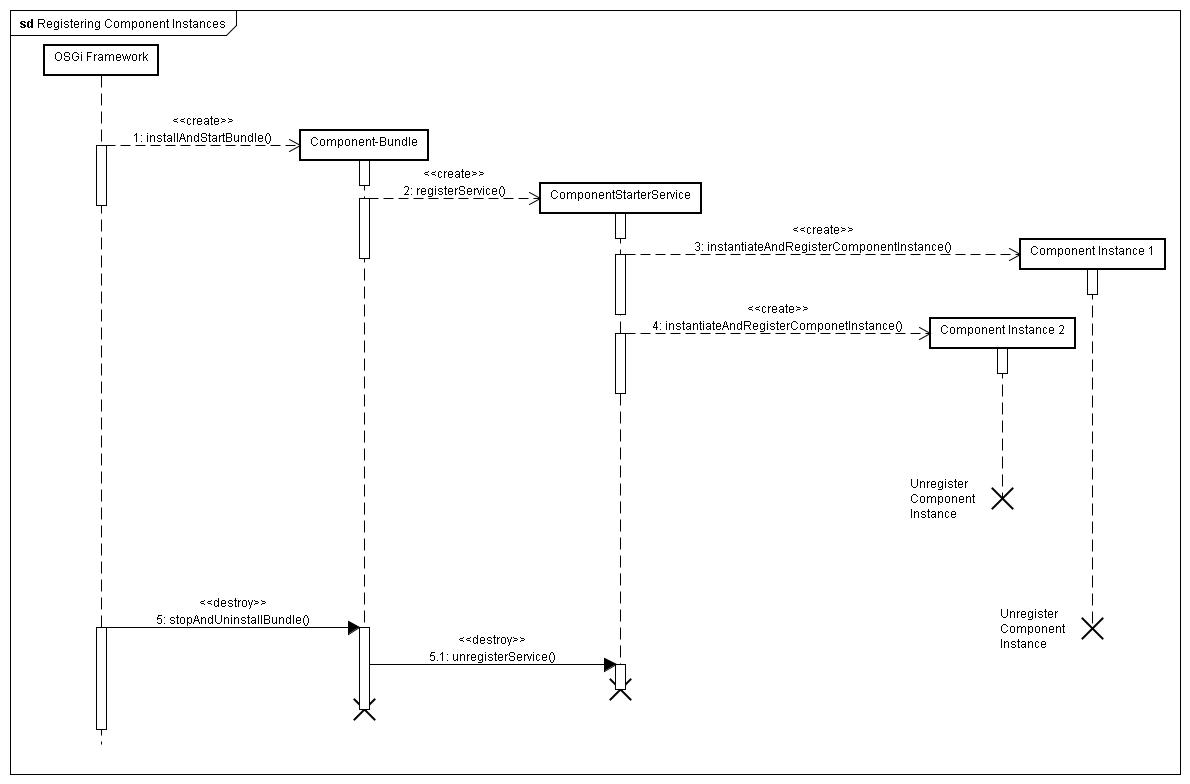
\includegraphics[width=1.2\textwidth,
		angle=90]{Bilder/sd_registering_component_instances.jpg}}
	\caption{Registering Component Instances}
	\label{fig:registering_component_instances}
\end{figure}

\paragraph{The ID Service}
\label{sec:id_service}
This service enables the unique identification of every instantiated and registered component
within the Component Framework, which is not provided by the OSGi Framework, but needed to realize
the ``Running multiple Instances of a Block'' requirement.

Within the OSGi Framework each bundle is identified by its symbolic name and version and the
registered services do not have to be identified at all. Most applications only need to know that
there is a service which can be used and hence do not have to distinguish between various service
implementations. That is different within the Component Framework, as multiple instances of the
same component, which all implement the same service, can be started. Therefore, the underlying OSGi
Framework does not provide the necessary means to clearly distinguish multiple instances of the
same component.

Hence, the ID Service provides an interface for getting a unique ID for a component instance within
the context of a project (see Section \ref{sec:project}). That means that the service produces an
ID which was not used so far for the given project name.

\subsubsection{Communication and Data Exchange (Requirements 2 and 8)}
\label{sec:communication}
This section deals with the services which were adapted and/or implemented to enable communication
and data exchange between components and to therewith fulfill Requirement 2 ``Data Access and
Processing'' and Requirement 8 ``Event Management'' (see Section \ref{chapter:requirements}).

\paragraph{Background}
For better understanding, this section describes the fundamentals of the Wire Admin and Event Admin
services, which are used and adapted to realize the ``Data Access and Processing'' and the ``Event
Management'' requirements.
Both, the Wire Admin and Event Admin services should provide the functionality to exchange data
between components and bundles respectively. Therefore, a system of ``Messaging
Channels'' is introduced, which is described as follows \cite{Hohpe2003}:

\msQuote{When two applications want to exchange data, they do so by sending the
data through a channel that connects the two. The application sending the data
may not know which application will receive the data. However, by selecting a
particular channel on which to send the data, the sender knows that the
receiver will be one that is looking for that sort of data by looking for it on
that channel. In this way, the applications that produce shared data have a way
to communicate with those that wish to consume it.}

Although this description speaks of applications the statements can be
perfectly mapped to components.

Within such a messaging system there can exist multiple types of channels.
The OSGi Framework uses two variants, namely ``Datatype'' and
``Publish-Subscribe'' channels.

\subparagraph{Datatype channel}
In the case of the ``Wire Admin Service'', OSGi specifies a variant of a datatype
channel.

The definition of a datatype channel says that all messages that are exchanged
via this channel have to be of the same data type \cite{Hohpe2003}. Being so restrictive makes
it easy for the receiver to handle the message and extract the necessary information. OSGi
is not that restrictive and allows to specify a set of data types for each channel.
Both, the producer and consumer of messages can specify their preferred data types
and can therefore react by sending messages in the best matching format that can
be handled by the sending and receiving component.

\subparagraph{Publish-Subscribe channel}
The Event Admin service, contained in the OSGi specification, uses the
publish-subscribe mechanism to exchange data.

\msQuote{A Publish-Subscribe Channel works like this: It has one input channel
that splits into multiple output channels, one for each subscriber. When an
event is published into the channel, the Publish-Subscribe Channel delivers a
copy of the message to each of the output channels.}

Within OSGi this kind of channel \cite{Hohpe2003} is realized as follows:

The publisher sends the event with a unique identifier, the so-called ``Topic''
via the ``Event Admin Service'' and the subscribers register so-called ``Event Handlers''
for the exact same event topic. That means that every Event Handler that is
registered for the appropriate topic receives the event.

\paragraph{Wire Admin Service}
\label{sec:wire_admin}
In order to exchange data between components and therewith realize the processing part of
Requirement 2 ``Data Access and Processing'' the Wire Admin Service is used. This service provides
methods to create so-called ``Wires'' between data ``Producers'' and ``Consumers''. To prepare and
enable the exchange of data between components, each of them has to implement the producer and
consumer interfaces and register these service implementations at the service registry. The
registration takes an additional input parameter, called ``persistent id'', in order to create the
wires later on and to establish the correct mapping between producer, consumer and the connection or
the wire respectively.

Furthermore, producer and consumer can specify a list of data types, which they
prefer to process. This enables producer components to send data to various
consumers, with respect to their preferred data type.

The wires which finally connect the two components can be initialized at any
time, even before the corresponding producers and consumers are registered.
This behavior is established by using the persistent ids of the two
connection endpoints as wire initialization parameters and hence producing a
unique mapping.

A wire is in the connected state as soon as both, the producer and consumer,
services are registered. Each time a connection is established, producer and
consumer are informed about the existing connected wires. Data transfer finally
can be achieved either by sending data through wires, which is done by
the producer, or by consumers actively polling data.

\subparagraph{Extensions of the Wire Admin Service by the Component Framework}
The Component Framework encapsulates the functionality of the OSGi Wire Admin Service and extends
it with special functionality.

For this purpose it implements methods for creating and deleting wires between two components,
deleting all wires of a component, for example if a component is stopped, and some more methods for
dealing with the persistent ID of a component. This ID must be unique within the Component
Framework and therefore consists of the unique project name and the component ID, which is produced
by the ID Service and is unique within the context of a project.

Within the framework every component acts as ``Producer'' and ``Consumer'', which enables a
bidirectional connection between components (see Figure \ref{fig:component_wire_admin}). The
sending and receiving of data is handled via the consumer and producer methods, which have to be
implemented for each component. In order to receive data and process it correctly knowledge about
the data-format is indispensable. This is a small limitation to the loose coupling of components,
but that is a limitation every service oriented architecture has to deal with and is in most
scenarios solved by using a communication standard that is based on XML (see Section
\ref{sec:service_oriented_architecture}).

\begin{figure}
	\centering
		\fbox{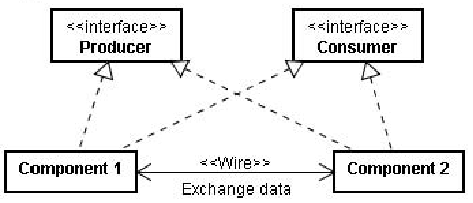
\includegraphics{Bilder/component_wire_admin.pdf}}
	\caption{Producer-Consumer Connection}
	\label{fig:component_wire_admin}
\end{figure}

As the Wire Admin and the Component Wire Admin respectively do not make any constraints on the data
exchange format, an XML based solution would be applicable for the Component Framework and the Wire
Admin Service as well, but was not implemented within the context of this master thesis.

Summing up, the Wire Admin service provides methods for exchanging data and hence realizes the
data processing part of Requirement 2, but also assumes a stronger connection and dependency between
components.

\paragraph{Event Admin Service}
\label{sec:event_admin}
The Event Admin Service provides the functionality for sending and receiving events throughout the
OSGi Framework and for realizing Requirement 8 ``Event Management''. In order to use these methods,
the Equinox implementation of the Event Admin Service has to be installed and started within the
framework. After the successful launch of the bundle, the Event Admin can be requested at the
service registry and used.

If a bundle or component respectively wants to receive and handle events, the Event Handler interface
has to be implemented and the appropriate class has to be registered at the registry. In order to
filter the events that are received by the Event Handler, the registration method takes an additional
parameter, which contains a list of properties. One of these properties defines the so-called topics,
which are nothing else than unique event identifiers within the Component and OSGi Framework
respectively, and therefore allow the filtering of single events or even sets of events.

As events are most commonly used to inform interested components about every kind of ``changes'', the
amount of information or data that is transferred is rather small. That means that the Event Admin
Service is not intended for exchanging bigger amounts of data. This is the place where the Wire Admin
Service comes into play.

\subparagraph{Event Information - An Extension to the Event Admin Service}
The event management system within the OSGi Framework requires event publishers and event
consumers, so-called ``Event Handlers''. In order to receive and process events from components,
which are unknown to the event handler, the sending component has to provide information about
them. For this purpose the ``Event Information Service'' was implemented.

That means that every component within the Component Framework, which wants to send events, has to
implement an ``Event Information'' object, which exposes human readable information about the
events, and register it at the service registry. The event information specifies the previously
described event topic, which is used as event identifier and various properties, which provide
additional information or data about when the event exactly is fired and how to handle it.

Figure \ref{fig:event_information_display} displays a simple example for a calculation result
event, which contains the name, description and topic of the event as well as the ``calculation
result'' property with its description, the identifying key, the default value and the type of the
value.

\begin{figure}
	\centering
		\fbox{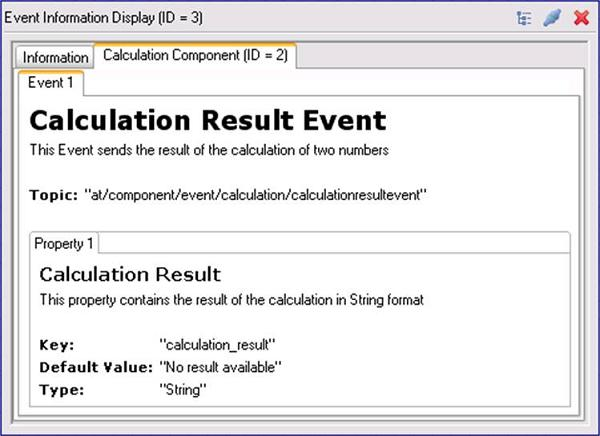
\includegraphics[width=0.6\textwidth]{Bilder/event_information_display.jpg}}
	\caption{Event Information Display}
	\label{fig:event_information_display}
\end{figure}

\subsubsection{Component Service (Requirements 4, 6 and 7)}
The ``Component Service'' finally constitutes the most powerful tool and provides a kind of management
agent (see Section \ref{label_life_cycle_layer}) for the Component Framework.

First of all this service recognizes all components and their bundles respectively which are started
with the OSGi Framework. As a second feature it provides methods for installing and uninstalling
component bundles as well as starting and stopping component instances (cf. Requirement 4 ``Running
multiple Instances of a Block''). The framework also takes care of the parent child relationship of
components and stops all child components as soon as a parent component is stopped. That means that
the component service provides a life-cycle management for components, enables the hot deployment
of new components within the Component Framework (cf. Requirement 7 ``Hot Deployment and Life-cycle
Management'').

Furthermore, the component service exposes methods for creating, saving, loading and deploying
projects. That means that the end user can reuse projects within other projects. Hence, Requirement
6 ``Reusability of Groups'' (see Section \ref{chapter:requirements}) is fulfilled and the monitor
for multiple airplanes (see Section \ref{sec:scenario}) can be implemented by first of all creating
a project for a single airplane and then integrating multiple instances of this project within a
bigger project which is adaptable to an arbitrary number of airplanes.

Another important aspect to mention about the component service and the saving
and loading of projects is, that every component can save data for reinitializing
the component during the loading process of a project. Two methods have to be
implemented to get this functionality. One for saving the data, which is called
during the saving process of the project and one for initializing the component.

As every service that is registered at the OSGi Service Registry (see Section
\ref{label_osgi_framework}) the Component Service is available throughout the entire OSGi as well as
Component Framework. Therefore, the exposed methods can be accessed by every component and enable
them to control the framework. As a second consequence the framework is absolutely independent of it's
graphical representation and the user interface. That means that the user interface which was
designed for the master thesis is just one simple example of doing it and therefore can be easily
enhanced or replaced.

\subsubsection{Component Log Service (Requirement 9)}
The ``Component Log Service'' encapsulates the log service of Eclipse Equinox and provides a simple interface for
logging all kinds of information (cf. Requirement 9 ``Logging''). It instantiates a logger which
writes the information into a log-file, which is located within the program folder. Additionally it is possible to implement
the ``IComponentLogService'' interface and add a different kind of logger, which for example prints
the information onto the console or updates the user interface of a running component.

\subsection{Extending the Component Framework (Requirement 3)}
\label{sec:extensibility}

This section deals with the development of custom components which can be managed by the Component
Framework, exchange data with other components and process events (cf. Requirement 3
``Extensibility'').

\subsubsection{Introduction}
To simplify the process of developing new components, which run within the
implemented framework, a ``New Component''-Wizard is provided as
Eclipse plug-in (see Figure \ref{fig:new_component_wizard}). This wizard only needs few inputs and
creates an Eclipse plug-in project targeted to the chosen OSGi Framework, which already
includes the basic Java classes, needed for a simple component (see Figure
\ref{fig:new_component_wizard_class_diagram}).

\begin{figure}
	\centering
		\fbox{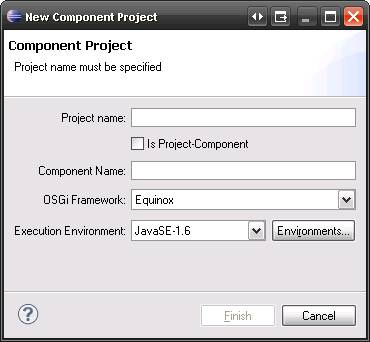
\includegraphics[width=0.6\textwidth]{Bilder/new_component_wizard.jpg}}
	\caption{New Component Wizard}
	\label{fig:new_component_wizard}
\end{figure}

\begin{figure}
	\centering
		\fbox{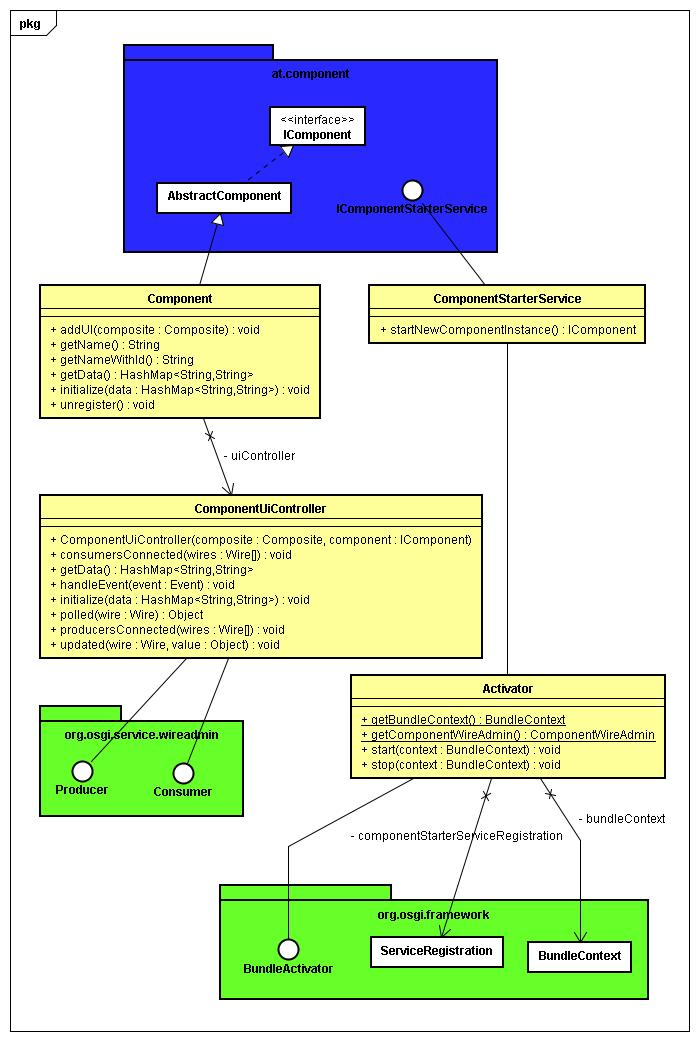
\includegraphics[width=0.8\textwidth]{Bilder/new_component_wizard_class_diagram.jpg}}
	\caption{New Component Wizard - Class Diagram}
	\label{fig:new_component_wizard_class_diagram}
\end{figure}

The Activator class implements the Bundle Activator interface of the OSGi
Framework and is the first class to be called by the framework during the
starting process of a bundle. Therefore, this class constitutes the perfect
place for registering the Component Starter Service, which is needed to start multiple instances of
a component, at the Service Registry (see Section \ref{label_osgi_framework}).

The ``Component'' class constitutes the main class of a component
implementation and provides fields for storing the name and the id of a
component, in order to identify the component instance within the running OSGi
Framework.

Furthermore, it is assumed that every component provides some
kind of user interface. Therefore, the component class provides a single
method, called ``addUI'', which provides a composite as parameter. This composite
constitutes the parent of the components user interface and hence is the place
to position buttons, input fields and all the other controls that are needed
to interact with the component. The applied mechanism can be compared with
viewparts in the RCP system of Eclipse \cite{eclipse_rcp}.

\subsubsection{Implementing the component}
\label{sec:component_implementation}
The starting point for implementing a new component is the
``ComponentUiController'' class, where the user interface class should be
instantiated (see Figure \ref{fig:new_component_wizard_class_diagram}). From that point onward
creating a component is like implementing a normal Java application according to the model-view-controller pattern.
Neither using multiple bundles for one component nor outsourcing a data model
for multiple components into a single bundle is a problem.

Therefore, simple data-display interfaces, like for example a component, which displays information
about the crew of a flight, can be done without using the Event Admin or the Component Wire Admin
(see Sections \ref{sec:event_admin} and \ref{sec:wire_admin}). As soon as a component
should react to some kind of events other components produce, or process data, which other
components are sending, these services have to be integrated and a better understanding of the OSGi
Framework is required. Nevertheless, the classes which are created by the ``New Component''-Wizard
and the services which are provided by the Component Framework -- like the adapted and extended
Wire Admin and Event Admin services -- already implement the necessary methods and just have to be
applied correctly.
\chapter{Validation of the Component Framework}
\label{chapter:applications}

In order to demonstrate the feasibility of the concepts of the framework and to meet Requirement
1 ``Simple User Interface'' (see Section \ref{chapter:requirements}), a test application which
utilizes and validates the Component Framework was implemented (cf. Section
\ref{sec:test_application}).

Furthermore, Mathias Breu� is using the Component Framework as basis for his bachelor thesis
\cite{scrumtool} to realize a complex component based (and therefore service oriented)
application (cf. Section \ref{sec:scrumtool}).

Finally, the Component Framework and the test application are analyzed in respect to the identified
requirements (cf. Section \ref{sec:solution_analysis}).

\section{Air Ambulance Test Application}
\label{sec:test_application}
To validate the developed Component Framework, a test application based on the air ambulance
scenario has been implemented. The test application can be seen as an interface to the Component
Framework using all its major functionalities (see Figure
\ref{fig:component_framework_user_interface}).

\begin{figure}
	\centering
		\fbox{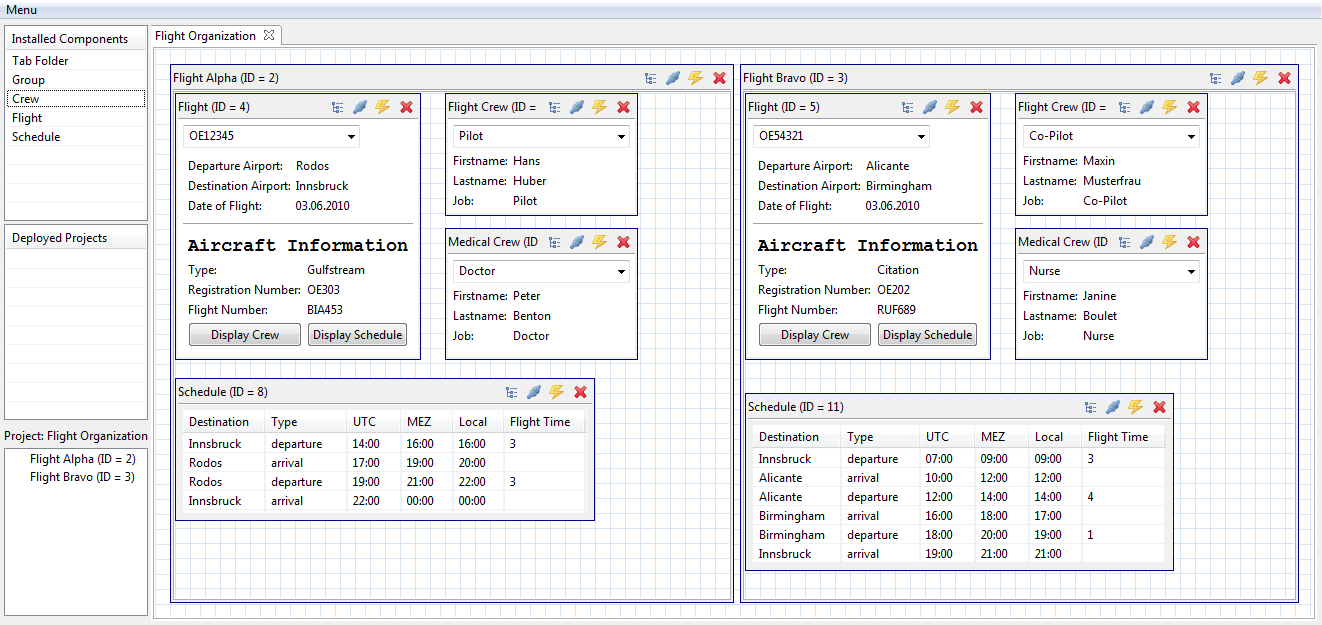
\includegraphics[width=1.2\textwidth,
		angle=90]{Bilder/test_application.png}}
	\caption{Test Application}
	\label{fig:component_framework_user_interface}
\end{figure}

The menu bar on top represents a direct link to the management agent functionality of the
component service and provides entries for installing component bundles and creating, saving, loading
and deploying projects.

On the left hand side the user interface provides information about installed component bundles,
deployed projects and the currently active components with respect to the selected project.
Additional context menus provide methods for uninstalling bundles and removing deployed projects.
Furthermore, the tables that display this information act as drag source. Therefore, other
components which implement a drop target can process the dragged data, as for example, the
``Group'' component does. It starts and displays the component and adds a menu bar for stopping the component again,
shifting it to another group component or connecting it with other components to directly exchange
data via the Component Wire Admin (see Section \ref{sec:wire_admin}).

The rest of the user interface is occupied by the working area, which is nothing else than a
tabfolder, where every tabitem constitutes a project. As soon as a new project is created and the
chosen project component is started, the user interface that is provided by the project component
(e.g., the group or tabfolder component) is placed on the tabitem. In the case of the displayed
example in Figure \ref{fig:component_framework_user_interface}, the project component is a
``Group'' component and the project is named ``Flight Organization''. Furthermore, the example
project has two child components, which are again ``Group'' components and hold the information of
two different flights. Therefore, the ``Flight Alpha'' and ``Flight Bravo'' components are populated
with different components which hold information about the flight, the airplane, the flight and
medical crew as well as about the detailed schedule. Both, the ``Crew'' and ``Schedule''
components receive their data from the ``Flight'' components by using the Wire and Event Admin
services (see Section \ref{sec:communication}).

\section{Scrumtool}
\label{sec:scrumtool}
For his bachelor thesis, Mathias Breu� developed a software product which is based on the described
test application and extends it with various custom components which should support Scrum teams
\cite{KS04} in the realization of software projects \cite{scrumtool}.

Figure \ref{fig:scrumtool} depicts the user interface of the test application which contains the
necessary custom components and extensively utilizes the provided complex components (see Section
\ref{sec:complex_components}) and hence the grouping and the launching of multiple
instances of a component functionality of the Component Framework. Furthermore, the scrumtool
transfers data from one component to the other by using the Wire Admin Service and requires the
Event Admin Service as well as the Event Information to propagate all kinds of events (see Section
\ref{sec:wire_admin}).

\begin{figure}
	\centering
		\fbox{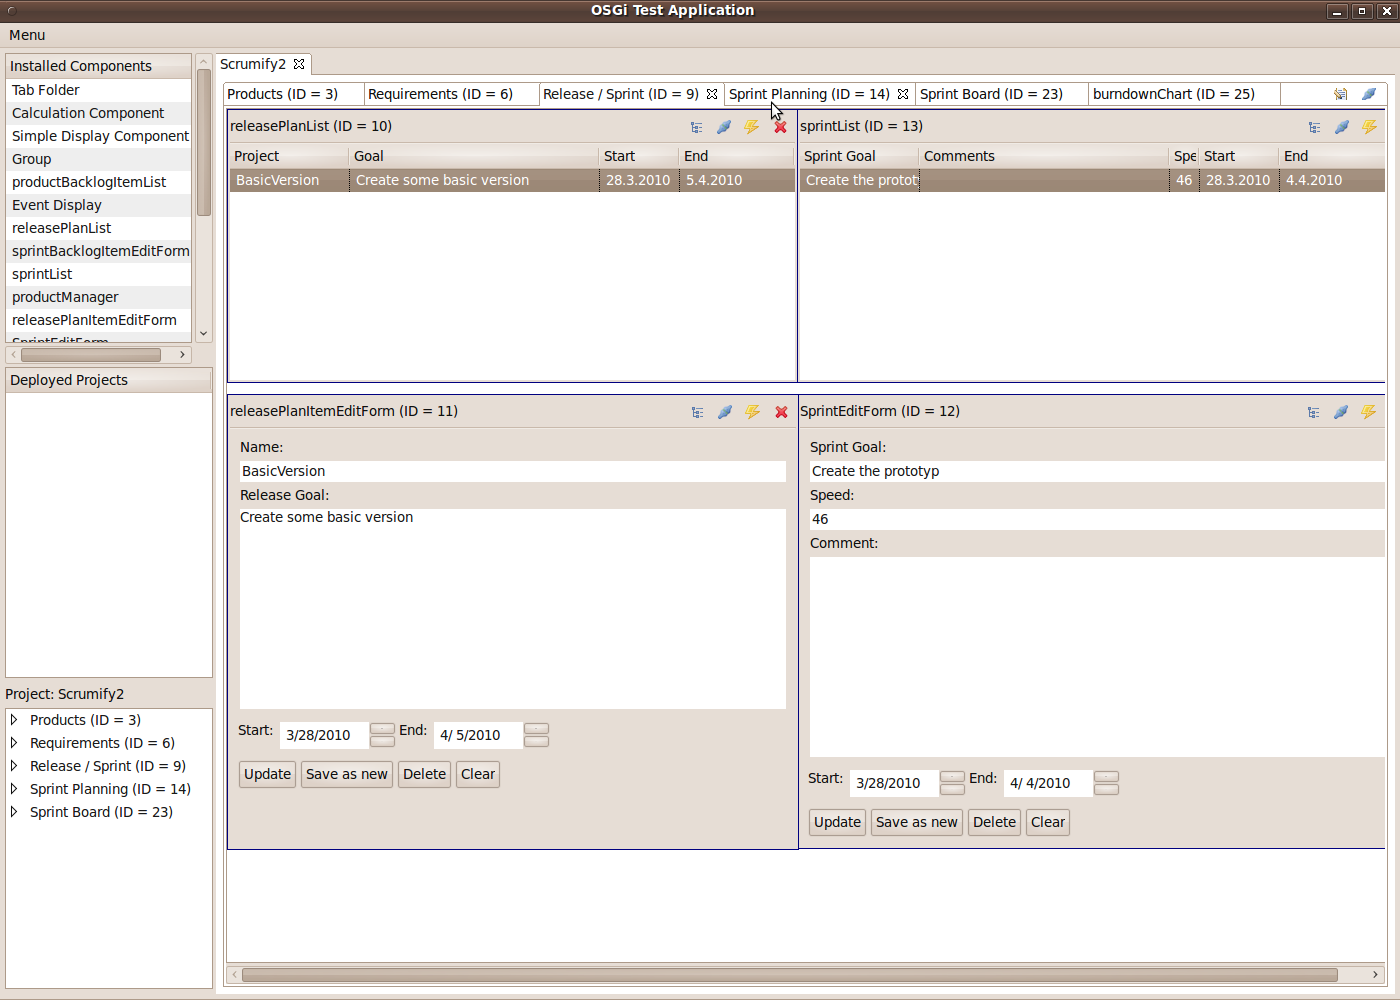
\includegraphics[width=0.98\textwidth]{Bilder/release_sprint.png}}
	\caption{Scrumtool}
	\label{fig:scrumtool}
\end{figure}

\section{Solution Analysis}
\label{sec:solution_analysis}
The ``Component Framework'' (see Section \ref{sec:component_framework}) was implemented to support
the identified requirements (see Section \ref{chapter:requirements}) and hence to provide a possible solution for
scenarios, like the air ambulance example which was introduced in Section \ref{sec:scenario}. The developed solution is
now analyzed to that effect.

\begin{itemize}
  \item \textbf{Simple User Interface}\newline The user interface which was developed for this master
  thesis is quite similar to the ones that are provided by the inspected mashup composers and adds
  the functionality to visually group components, to deploy these groups within other mashups or
  applications respectively and to install, start, stop and uninstall components. Summing up the
  user interface of the test application is easily operated and applies the popular drag and drop
  functions. Furthermore, it hides the complexity of the OSGi and Component Framework which
  encourages the user to create simple applications and mashups with a few mouse clicks.
  \item \textbf{Data Access and Processing}\newline As Java is the selected programming language and
  as the framework is highly extensible, components for most data sources can be easily implemented.
  That means that databases as well as Excel sheets, CSV files or even web services can be
  accessed.\newline However, the focus of this thesis was the implementation of a prototype framework
  and hence lacks many of these data access components. Anyhow, since the framework is easily
  extensible and provides a wizard for creating new components, additional data access components can
  be easily added.\newline In the context of data processing the Component Framework provides
  possibilities to directly connect two components via the Component Wire Admin (see Section
  \ref{sec:wire_admin}) or to publish events via the Event Admin and the Event Information Service
  (see Section \ref{sec:event_admin}) which are consumed by interested components. These mechanisms
  can be used to send and receive every kind of data and hence do not force the usage of a
  particular data format. However, it is possible to specify various preferred data formats, but if
  neither the data producer nor the consumer component can convert the data to one of these formats,
  an extra component has to be implemented, which performs the conversion.\newline That means that
  the Component Framework places the responsibility for eliminating data processing or compatibility
  problems on the end-user or component developer respectively.
  \item \textbf{Extensibility}\newline The Component Framework or the test application respectively
  provide a very limited number of pre-built blocks. Yet, these blocks offer powerful means for
  grouping components and reusing them within other applications in order to realize for example the
  monitoring of multiple airplanes in parallel (see Section \ref{sec:scenario}). Nevertheless, the
  framework has to be extended with custom blocks to make it applicable within specific usage
  scenarios.\newline To make the development of new components and hence the implementation of
  missing pre-built blocks and the extension of the Component Framework as easy as possible a wizard
  was implemented which generates the main classes and highlights the entry points for the custom
  code (see Section \ref{sec:component_implementation}). However, this requirement was already
  fulfilled by Microsoft Popfly and IBM Mashup Center and therefore does not constitute an advantage
  over existing mashup composer tools.
  \item \textbf{Running Multiple Instances of a Block}\newline As you can see in Section
  \ref{sec:test_application} the Component Framework allows the launching of multiple instances of
  components (e.g., the ``Flight'' or ``Crew'' components). This is realized by extending the OSGi
  Framework with the Component Starter and ID Service (see Section \ref{sec:component_starter_service}).
  \item \textbf{Grouping of Blocks}\newline The Component Framework provides great support for
  grouping of blocks via two different mechanisms (see Section \ref{sec:project}).\newline The first
  one is the concept of ``projects'', which can be compared to ``sites'' within IBM Mashup Center.
  For each project a tab is created which is filled with the chosen ``project component''. The test
  application therefore implements complex components (the ``Group'' and ``TabFolder'' components)
  which provide the possibility to drag and drop and arrange every kind of child component on
  them.\newline The second mechanism enables the grouping of components within projects. Therefore,
  the framework implements a parent child relationship and the components, which want to provide
  grouping functionality have to implement a form of display for the child components, like the
  described working area or a simple tabfolder, where each child constitutes a tabitem. That means
  that complex components can be used as ``project components'' and as child components of a
  ``project component'' and hence enable the nesting and grouping of components (cf. ``Flight Alpha''
  and ``Flight Bravo'' in Figure \ref{fig:component_framework_user_interface}).\newline Therefore,
  Requirement 5 ``Grouping of Blocks'' is fully supported and can be further enhanced by custom
  components.
  \item \textbf{Reusability of Groups}\newline Reusability of groups within the Component
  Framework is supported by enabling the deployment of projects within other projects or
  applications respectively. As soon as they are deployed, these projects are handled like simple
  groups within the new project and support the same life-cycle. Hence, they can be installed,
  started, stopped and uninstalled.
  \item \textbf{Hot Deployment and Life-cycle Management}\newline By using OSGi as underlying
  technological platform and extending it with the ``Component Service'', hot deployment and
  life-cycle management are enabled. Within the test application components are started by simply
  dropping them on a ``Group'' or ``TabFolder'' component and can be stopped at any time by using
  the provided menu bar, which is attached to every single component.
  \item \textbf{Event Management}\newline The event management service of the Component Framework
  encapsulates the basic functionality that is provided by the OSGi Framework and therefore enables
  the sending of events as well as the registration of components as Event Handlers for either
  single specific events or for groups of events. Furthermore, it extends the event mechanism by
  providing interfaces which should be implemented to expose human readable information about
  events (see Section \ref{sec:event_admin}). This alleviates the implementation of Event
  Handlers and makes the events processable correctly.
  \item \textbf{Logging}\newline The logging mechanism of the Component Framework enables the
  logging of errors, warnings and simple information, which can be analyzed by the component
  developers and reused to conduct data and process mining methods.
\end{itemize}

\chapter{Summary}
\label{chapter:summary}

The evaluation of three mashup composers (see Chapter \ref{chapter:evaluation}), namely
``Microsoft Popfly'', ``Yahoo Pipes'' and ``IBM Mashup Center'' revealed, besides strengths like
the user interface, some major problems or shortcomings respectively, which are not solved or
implemented yet. Hence, requirements for a software product which integrates the identified
strengths and eliminates the weaknesses from the introduced evaluation criteria, are deduced (see
Chapter \ref{chapter:requirements}). Chapter \ref{chapter:osgi} introduces the Component Framework,
which is based on approved technologies and extends them with the required functionality to support
the identified requirements. Finally, Chapter \ref{chapter:applications} validates the introduced
framework by implementing a test application which can be seen as an interface to the Component
Framework and hence uses all its major functionalities.

\section{Conclusion}

To sum up, the Component Framework provides means to easily develop mashups and applications on the
basis of approved technologies like Java and OSGi. It eliminates most weaknesses of the evaluated
mashup composers by providing an extensive and further extensible grouping functionality of single
components, by making these groups reusable within other mashups, by integrating a life-cycle
management for single components as well as groups, by implementing an event management system
which enables a loosely coupled communication between components and by providing a logging
mechanism which provides a source for important feedback for the component developer and enables
data mining.

The implemented prototype application, which can be seen as an interface to the Component Framework,
finally provides methods to drag, drop and arrange components on a working area, to group components
within various forms of display, to connect components, in order to exchange, aggregate and process
data and to save and reuse the created projects.

Furthermore, a plug-in for Eclipse is provided, which alleviates the process of implementing custom
components and hence extend and enhance the framework or the prototype application respectively.

Hence, the developed solution provides better means than existing mashup composer tools to fulfill
the requirements of the introduced air ambulance scenario as well as of similar examples.

\section{Outlook}

As master theses are in most cases limited in time and resources that can be spent on it, the
Component Framework and the prototype application which were developed for this thesis indeed
fulfill the identified requirements, but still have great potentials to be further extended and
enhanced. A XML-based communication standard which is newly implemented or adapted from existing
service oriented technologies or the creation of a central service repository would be only two of
many interesting extensions.

\listoffigures
\listoftables

\bibliographystyle{alpha}
\bibliography{literature}

\end{document}
